% **************************************************************************************************************
% A Classic Thesis Style
% An Homage to The Elements of Typographic Style
%
% Copyright (C) 2015 André Miede http://www.miede.de
%
% If you like the style then I would appreciate a postcard. My address 
% can be found in the file ClassicThesis.pdf. A collection of the 
% postcards I received so far is available online at 
% http://postcards.miede.de
%
% License:
% This program is free software; you can redistribute it and/or modify
% it under the terms of the GNU General Public License as published by
% the Free Software Foundation; either version 2 of the License, or
% (at your option) any later version.
%
% This program is distributed in the hope that it will be useful,
% but WITHOUT ANY WARRANTY; without even the implied warranty of
% MERCHANTABILITY or FITNESS FOR A PARTICULAR PURPOSE.  See the
% GNU General Public License for more details.
%
% You should have received a copy of the GNU General Public License
% along with this program; see the file COPYING.  If not, write to
% the Free Software Foundation, Inc., 59 Temple Place - Suite 330,
% Boston, MA 02111-1307, USA.   
%
% **************************************************************************************************************
\RequirePackage{fix-cm} % fix some latex issues see: http://texdoc.net/texmf-dist/doc/latex/base/fixltx2e.pdf
\documentclass[ oneside,openany,titlepage,numbers=noenddot,headinclude,%1headlines,% letterpaper a4paper
                footinclude=true,cleardoublepage=empty,abstractoff, % <--- obsolete, remove (todo)
                BCOR=5mm,paper=a4,fontsize=11pt,%11pt,a4paper,%
                spanish,american%
                ]{scrreprt}

%********************************************************************
% Note: Make all your adjustments in here
%*******************************************************
% ****************************************************************************************************
% classicthesis-config.tex 
% formerly known as loadpackages.sty, classicthesis-ldpkg.sty, and classicthesis-preamble.sty 
% Use it at the beginning of your ClassicThesis.tex, or as a LaTeX Preamble 
% in your ClassicThesis.{tex,lyx} with % ****************************************************************************************************
% classicthesis-config.tex 
% formerly known as loadpackages.sty, classicthesis-ldpkg.sty, and classicthesis-preamble.sty 
% Use it at the beginning of your ClassicThesis.tex, or as a LaTeX Preamble 
% in your ClassicThesis.{tex,lyx} with % ****************************************************************************************************
% classicthesis-config.tex 
% formerly known as loadpackages.sty, classicthesis-ldpkg.sty, and classicthesis-preamble.sty 
% Use it at the beginning of your ClassicThesis.tex, or as a LaTeX Preamble 
% in your ClassicThesis.{tex,lyx} with \input{classicthesis-config}
% ****************************************************************************************************  
% If you like the classicthesis, then I would appreciate a postcard. 
% My address can be found in the file ClassicThesis.pdf. A collection 
% of the postcards I received so far is available online at 
% http://postcards.miede.de
% ****************************************************************************************************


% ****************************************************************************************************
% 0. Set the encoding of your files. UTF-8 is the only sensible encoding nowadays. If you can't read
% äöüßáéçèê∂åëæƒÏ€ then change the encoding setting in your editor, not the line below. If your editor
% does not support utf8 use another editor!
% ****************************************************************************************************
\PassOptionsToPackage{utf8}{inputenc}
	\usepackage{inputenc}

% ****************************************************************************************************
% 1. Configure classicthesis for your needs here, e.g., remove "drafting" below 
% in order to deactivate the time-stamp on the pages
% ****************************************************************************************************
\PassOptionsToPackage{listings,eulerchapternumbers,%eulermath,%drafting,%
                      pdfspacing,floatperchapter,%linedheaders,%
                      beramono,
                      subfig,parts,dottedtoc}{classicthesis}                                        
% ********************************************************************
% Available options for classicthesis.sty 
% (see ClassicThesis.pdf for more information):
% drafting
% parts nochapters linedheaders
% eulerchapternumbers beramono eulermath pdfspacing minionprospacing
% tocaligned dottedtoc manychapters
% listings floatperchapter subfig
% ********************************************************************


% ****************************************************************************************************
% 2. Personal data and user ad-hoc commands
% ****************************************************************************************************
\newcommand{\myTitle}{Problema isoperimétrico en el espacio euclídeo. Representación de información imprecisa en base de datos NoSQL\xspace}
\newcommand{\mySubtitle}{ \xspace}
%\newcommand{\mySubtitle}{Resolución problema isoperimétrico y propuesta MongoDB\xspace}
\newcommand{\myWork}{Trabajo Fin de Grado}
\newcommand{\myDegree}{Doble Grado en Ingeniería Informática y Matemáticas\xspace}
\newcommand{\myName}{Sergio Padilla López\xspace}
\newcommand{\myProf}{César Rosales Lombardo\xspace}
\newcommand{\myOtherProf}{Juan Miguel Medina Rodríguez\xspace}
%\newcommand{\mySupervisor}{Put name here\xspace}
\newcommand{\myFaculty}{Facultad de Ciencias\xspace}
\newcommand{\myOtherFaculty}{Escuela Técnica Superior de Ingenierías Informática y de Telecomunicación\xspace}
\newcommand{\myOtherFacultyA}{Escuela Técnica Superior de Ingenierías\xspace}
\newcommand{\myOtherFacultyB}{Informática y de Telecomunicación\xspace}
%\newcommand{\myDepartment}{Put data here\xspace}
\newcommand{\myUni}{Universidad de Granada\xspace}
\newcommand{\myLocation}{Granada\xspace}
\newcommand{\myTime}{Junio de 2018\xspace}
%\newcommand{\myVersion}{version 4.2\xspace}

% ********************************************************************
% Setup, finetuning, and useful commands
% ********************************************************************
\newcounter{dummy} % necessary for correct hyperlinks (to index, bib, etc.)
\newlength{\abcd} % for ab..z string length calculation
\providecommand{\mLyX}{L\kern-.1667em\lower.25em\hbox{Y}\kern-.125emX\@}
\newcommand{\ie}{i.\,e.}
\newcommand{\Ie}{I.\,e.}
\newcommand{\eg}{e.\,g.}
\newcommand{\Eg}{E.\,g.} 
% ****************************************************************************************************


% ****************************************************************************************************
% 3. Loading some handy packages
% ****************************************************************************************************
% ******************************************************************** 
% Packages with options that might require adjustments
% ******************************************************************** 
%\PassOptionsToPackage{ngerman,american}{babel}   % change this to your language(s)
% Spanish languages need extra options in order to work with this template
\PassOptionsToPackage{spanish,es-lcroman}{babel}
	\usepackage{babel}                  

\usepackage{csquotes}
\PassOptionsToPackage{%
    backend=biber, %instead of bibtex
	%backend=bibtex8,
	bibencoding=ascii,%
	language=auto,%
	style=numeric-comp,%
    %style=authoryear, % Author 1999, 2010
    %bibstyle=authoryear,dashed=false, % dashed: substitute rep. author with ---
    sorting=nyt, % name, year, title
    maxbibnames=3, % default: 3, et al.
    %backref=true,%
    natbib=true % natbib compatibility mode (\citep and \citet still work)
}{biblatex}
    \usepackage{biblatex}

%\PassOptionsToPackage{fleqn}{amsmath}       % math environments and more by the AMS 
    \usepackage{amsmath}
    
\usepackage{amssymb}

% ******************************************************************** 
% General useful packages
% ******************************************************************** 
\PassOptionsToPackage{T1}{fontenc} % T2A for cyrillics
    \usepackage{fontenc}     
\usepackage{textcomp} % fix warning with missing font shapes
\usepackage{scrhack} % fix warnings when using KOMA with listings package          
\usepackage{xspace} % to get the spacing after macros right  
\usepackage{mparhack} % get marginpar right
\usepackage{fixltx2e} % fixes some LaTeX stuff --> since 2015 in the LaTeX kernel (see below)
%\usepackage[latest]{latexrelease} % will be used once available in more distributions (ISSUE #107)
\PassOptionsToPackage{printonlyused,smaller}{acronym} 
    \usepackage{acronym} % nice macros for handling all acronyms in the thesis
    %\renewcommand{\bflabel}[1]{{#1}\hfill} % fix the list of acronyms --> no longer working
    %\renewcommand*{\acsfont}[1]{\textsc{#1}} 
    \renewcommand*{\aclabelfont}[1]{\acsfont{#1}}
 
    
% *********************************************
% Paquete todonotes. Paquete para intrducir notas en texto pdf generado
%**********************************************
% Para activar las notas descomentar la linea siguiente y comentar la segunda
% Para desactivar las notas descomentar la linea segunda y comentar la primera
%\usepackage[textwidth=2.2cm]{todonotes}
%\usepackage[disable]{todonotes}
%\listoftodos
% Copiar y modificar los ejemplos de notas de abajo y ubicarlos donde queramos que 
% aparezca la nota

%\todo[author=JM,color=blue!40,inline,caption={Texto para el indice}]{Entre llaves introduces el texto de la anotación}
%\todo[author=Sergio,color=green!40,inline,caption={Carlos: Anotaciones de Sergio}]{Entre llaves introduces el texto de la anotacion}

% ****************************************************************************************************


% ****************************************************************************************************
% 4. Setup floats: tables, (sub)figures, and captions
% ****************************************************************************************************
\usepackage{tabularx} % better tables
    \setlength{\extrarowheight}{3pt} % increase table row height
\newcommand{\tableheadline}[1]{\multicolumn{1}{c}{\spacedlowsmallcaps{#1}}}
\newcommand{\myfloatalign}{\centering} % to be used with each float for alignment
\usepackage{caption}
% Thanks to cgnieder and Claus Lahiri
% http://tex.stackexchange.com/questions/69349/spacedlowsmallcaps-in-caption-label
% [REMOVED DUE TO OTHER PROBLEMS, SEE ISSUE #82]    
%\DeclareCaptionLabelFormat{smallcaps}{\bothIfFirst{#1}{~}\MakeTextLowercase{\textsc{#2}}}
%\captionsetup{font=small,labelformat=smallcaps} % format=hang,
\captionsetup{font=small} % format=hang,
\usepackage{subfig}  
% ****************************************************************************************************

%\PassOptionsToPackage{usenames,dvipsnames}{xcolor}

% ****************************************************************************************************
% 5. Setup code listings
% ****************************************************************************************************
\usepackage{listings} 
%\lstset{emph={trueIndex,root},emphstyle=\color{BlueViolet}}%\underbar} % for special keywords
\lstset{language=bash,%
    morekeywords={PassOptionsToPackage,selectlanguage},
    keywordstyle=\color{black},%\bfseries,
    basicstyle=\small\color{Periwinkle}\ttfamily,
    identifierstyle=\color{black},
    commentstyle=\itshape\color{OliveGreen},
    stringstyle=\color{Thistle},
    numbers=left,%none,%left,%
    numberstyle=\color{Gray}\scriptsize,%\tiny
    stepnumber=1,
    numbersep=8pt,
    showstringspaces=false,
    breaklines=true,
    %frameround=ftff,
    %frame=single,
    belowcaptionskip=.75\baselineskip
    %frame=L
} 
% ****************************************************************************************************             


% ****************************************************************************************************
% 6. PDFLaTeX, hyperreferences and citation backreferences
% ****************************************************************************************************
% ********************************************************************
% Using PDFLaTeX
% ********************************************************************
\PassOptionsToPackage{pdftex,hyperfootnotes=false,pdfpagelabels}{hyperref}
    \usepackage{hyperref}  % backref linktocpage pagebackref
\pdfcompresslevel=9
\pdfadjustspacing=1 
\PassOptionsToPackage{pdftex}{graphicx}
    \usepackage{graphicx} 
 

% ********************************************************************
% Hyperreferences
% ********************************************************************
\hypersetup{%
    %draft, % = no hyperlinking at all (useful in b/w printouts)
    colorlinks=true, linktocpage=true, pdfstartpage=3, pdfstartview=FitV,%
    % uncomment the following line if you want to have black links (e.g., for printing)
    %colorlinks=false, linktocpage=false, pdfstartpage=3, pdfstartview=FitV, pdfborder={0 0 0},%
    breaklinks=true, pdfpagemode=UseNone, pageanchor=true, pdfpagemode=UseOutlines,%
    plainpages=false, bookmarksnumbered, bookmarksopen=true, bookmarksopenlevel=1,%
    hypertexnames=true, pdfhighlight=/O,%nesting=true,%frenchlinks,%
    urlcolor=RoyalBlue, linkcolor=NavyBlue, citecolor=Plum, %pagecolor=RoyalBlue,%
    %urlcolor=Black, linkcolor=Black, citecolor=Black, %pagecolor=Black,%
    pdftitle={\myTitle},%
    pdfauthor={\textcopyright\ \myName, \myUni, \myFaculty},%
    pdfsubject={},%
    pdfkeywords={},%
    pdfcreator={pdfLaTeX},%
    pdfproducer={LaTeX with hyperref and classicthesis}%
}   

% ********************************************************************
% Setup autoreferences
% ********************************************************************
% There are some issues regarding autorefnames
% http://www.ureader.de/msg/136221647.aspx
% http://www.tex.ac.uk/cgi-bin/texfaq2html?label=latexwords
% you have to redefine the makros for the 
% language you use, e.g., american, ngerman
% (as chosen when loading babel/AtBeginDocument)
% ********************************************************************
\makeatletter
\@ifpackageloaded{babel}%
    {%
       \addto\extrasspanish{%
			\renewcommand*{\figureautorefname}{Figura}%
			\renewcommand*{\tableautorefname}{Tabla}%
			\renewcommand*{\partautorefname}{Parte}%
			\renewcommand*{\chapterautorefname}{Capítulo}%
			\renewcommand*{\sectionautorefname}{Sección}%
			\renewcommand*{\subsectionautorefname}{Sección}%
			\renewcommand*{\subsubsectionautorefname}{Sección}%     
                }%
       \addto\extrasamerican{%
			\renewcommand*{\figureautorefname}{Figure}%
			\renewcommand*{\tableautorefname}{Table}%
			\renewcommand*{\partautorefname}{Part}%
			\renewcommand*{\chapterautorefname}{Chapter}%
			\renewcommand*{\sectionautorefname}{Section}%
			\renewcommand*{\subsectionautorefname}{Section}%
			\renewcommand*{\subsubsectionautorefname}{Section}%     
                }%
       \addto\extrasngerman{% 
			\renewcommand*{\paragraphautorefname}{Absatz}%
			\renewcommand*{\subparagraphautorefname}{Unterabsatz}%
			\renewcommand*{\footnoteautorefname}{Fu\"snote}%
			\renewcommand*{\FancyVerbLineautorefname}{Zeile}%
			\renewcommand*{\theoremautorefname}{Theorem}%
			\renewcommand*{\appendixautorefname}{Anhang}%
			\renewcommand*{\equationautorefname}{Gleichung}%        
			\renewcommand*{\itemautorefname}{Punkt}%
                }%  
            % Fix to getting autorefs for subfigures right (thanks to Belinda Vogt for changing the definition)
            \providecommand{\subfigureautorefname}{\figureautorefname}%             
    }{\relax}
\makeatother


% ****************************************************************************************************
% 7. Last calls before the bar closes
% ****************************************************************************************************
% ********************************************************************
% Development Stuff
% ********************************************************************
\listfiles
%\PassOptionsToPackage{l2tabu,orthodox,abort}{nag}
%   \usepackage{nag}
%\PassOptionsToPackage{warning, all}{onlyamsmath}
%   \usepackage{onlyamsmath}

% ********************************************************************
% Last, but not least...
% ********************************************************************
\usepackage{classicthesis} 
% ****************************************************************************************************


% ****************************************************************************************************
% 8. Further adjustments (experimental)
% ****************************************************************************************************
% ********************************************************************
% Changing the text area
% ********************************************************************
%\linespread{1.05} % a bit more for Palatino
%\areaset[current]{312pt}{761pt} % 686 (factor 2.2) + 33 head + 42 head \the\footskip
%\setlength{\marginparwidth}{7em}%
%\setlength{\marginparsep}{2em}%

% ********************************************************************
% Using different fonts
% ********************************************************************
%\usepackage[oldstylenums]{kpfonts} % oldstyle notextcomp
%\usepackage[osf]{libertine}
%\usepackage[light,condensed,math]{iwona}
%\renewcommand{\sfdefault}{iwona}
%\usepackage{lmodern} % <-- no osf support :-(
%\usepackage{cfr-lm} % 
%\usepackage[urw-garamond]{mathdesign} <-- no osf support :-(
%\usepackage[default,osfigures]{opensans} % scale=0.95 
%\usepackage[sfdefault]{FiraSans}
% ****************************************************************************************************

\usepackage{diffcoeff}
% ****************************************************************************************************  
% If you like the classicthesis, then I would appreciate a postcard. 
% My address can be found in the file ClassicThesis.pdf. A collection 
% of the postcards I received so far is available online at 
% http://postcards.miede.de
% ****************************************************************************************************


% ****************************************************************************************************
% 0. Set the encoding of your files. UTF-8 is the only sensible encoding nowadays. If you can't read
% äöüßáéçèê∂åëæƒÏ€ then change the encoding setting in your editor, not the line below. If your editor
% does not support utf8 use another editor!
% ****************************************************************************************************
\PassOptionsToPackage{utf8}{inputenc}
	\usepackage{inputenc}

% ****************************************************************************************************
% 1. Configure classicthesis for your needs here, e.g., remove "drafting" below 
% in order to deactivate the time-stamp on the pages
% ****************************************************************************************************
\PassOptionsToPackage{listings,eulerchapternumbers,%eulermath,%drafting,%
                      pdfspacing,floatperchapter,%linedheaders,%
                      beramono,
                      subfig,parts,dottedtoc}{classicthesis}                                        
% ********************************************************************
% Available options for classicthesis.sty 
% (see ClassicThesis.pdf for more information):
% drafting
% parts nochapters linedheaders
% eulerchapternumbers beramono eulermath pdfspacing minionprospacing
% tocaligned dottedtoc manychapters
% listings floatperchapter subfig
% ********************************************************************


% ****************************************************************************************************
% 2. Personal data and user ad-hoc commands
% ****************************************************************************************************
\newcommand{\myTitle}{Problema isoperimétrico en el espacio euclídeo. Representación de información imprecisa en base de datos NoSQL\xspace}
\newcommand{\mySubtitle}{ \xspace}
%\newcommand{\mySubtitle}{Resolución problema isoperimétrico y propuesta MongoDB\xspace}
\newcommand{\myWork}{Trabajo Fin de Grado}
\newcommand{\myDegree}{Doble Grado en Ingeniería Informática y Matemáticas\xspace}
\newcommand{\myName}{Sergio Padilla López\xspace}
\newcommand{\myProf}{César Rosales Lombardo\xspace}
\newcommand{\myOtherProf}{Juan Miguel Medina Rodríguez\xspace}
%\newcommand{\mySupervisor}{Put name here\xspace}
\newcommand{\myFaculty}{Facultad de Ciencias\xspace}
\newcommand{\myOtherFaculty}{Escuela Técnica Superior de Ingenierías Informática y de Telecomunicación\xspace}
\newcommand{\myOtherFacultyA}{Escuela Técnica Superior de Ingenierías\xspace}
\newcommand{\myOtherFacultyB}{Informática y de Telecomunicación\xspace}
%\newcommand{\myDepartment}{Put data here\xspace}
\newcommand{\myUni}{Universidad de Granada\xspace}
\newcommand{\myLocation}{Granada\xspace}
\newcommand{\myTime}{Junio de 2018\xspace}
%\newcommand{\myVersion}{version 4.2\xspace}

% ********************************************************************
% Setup, finetuning, and useful commands
% ********************************************************************
\newcounter{dummy} % necessary for correct hyperlinks (to index, bib, etc.)
\newlength{\abcd} % for ab..z string length calculation
\providecommand{\mLyX}{L\kern-.1667em\lower.25em\hbox{Y}\kern-.125emX\@}
\newcommand{\ie}{i.\,e.}
\newcommand{\Ie}{I.\,e.}
\newcommand{\eg}{e.\,g.}
\newcommand{\Eg}{E.\,g.} 
% ****************************************************************************************************


% ****************************************************************************************************
% 3. Loading some handy packages
% ****************************************************************************************************
% ******************************************************************** 
% Packages with options that might require adjustments
% ******************************************************************** 
%\PassOptionsToPackage{ngerman,american}{babel}   % change this to your language(s)
% Spanish languages need extra options in order to work with this template
\PassOptionsToPackage{spanish,es-lcroman}{babel}
	\usepackage{babel}                  

\usepackage{csquotes}
\PassOptionsToPackage{%
    backend=biber, %instead of bibtex
	%backend=bibtex8,
	bibencoding=ascii,%
	language=auto,%
	style=numeric-comp,%
    %style=authoryear, % Author 1999, 2010
    %bibstyle=authoryear,dashed=false, % dashed: substitute rep. author with ---
    sorting=nyt, % name, year, title
    maxbibnames=3, % default: 3, et al.
    %backref=true,%
    natbib=true % natbib compatibility mode (\citep and \citet still work)
}{biblatex}
    \usepackage{biblatex}

%\PassOptionsToPackage{fleqn}{amsmath}       % math environments and more by the AMS 
    \usepackage{amsmath}
    
\usepackage{amssymb}

% ******************************************************************** 
% General useful packages
% ******************************************************************** 
\PassOptionsToPackage{T1}{fontenc} % T2A for cyrillics
    \usepackage{fontenc}     
\usepackage{textcomp} % fix warning with missing font shapes
\usepackage{scrhack} % fix warnings when using KOMA with listings package          
\usepackage{xspace} % to get the spacing after macros right  
\usepackage{mparhack} % get marginpar right
\usepackage{fixltx2e} % fixes some LaTeX stuff --> since 2015 in the LaTeX kernel (see below)
%\usepackage[latest]{latexrelease} % will be used once available in more distributions (ISSUE #107)
\PassOptionsToPackage{printonlyused,smaller}{acronym} 
    \usepackage{acronym} % nice macros for handling all acronyms in the thesis
    %\renewcommand{\bflabel}[1]{{#1}\hfill} % fix the list of acronyms --> no longer working
    %\renewcommand*{\acsfont}[1]{\textsc{#1}} 
    \renewcommand*{\aclabelfont}[1]{\acsfont{#1}}
 
    
% *********************************************
% Paquete todonotes. Paquete para intrducir notas en texto pdf generado
%**********************************************
% Para activar las notas descomentar la linea siguiente y comentar la segunda
% Para desactivar las notas descomentar la linea segunda y comentar la primera
%\usepackage[textwidth=2.2cm]{todonotes}
%\usepackage[disable]{todonotes}
%\listoftodos
% Copiar y modificar los ejemplos de notas de abajo y ubicarlos donde queramos que 
% aparezca la nota

%\todo[author=JM,color=blue!40,inline,caption={Texto para el indice}]{Entre llaves introduces el texto de la anotación}
%\todo[author=Sergio,color=green!40,inline,caption={Carlos: Anotaciones de Sergio}]{Entre llaves introduces el texto de la anotacion}

% ****************************************************************************************************


% ****************************************************************************************************
% 4. Setup floats: tables, (sub)figures, and captions
% ****************************************************************************************************
\usepackage{tabularx} % better tables
    \setlength{\extrarowheight}{3pt} % increase table row height
\newcommand{\tableheadline}[1]{\multicolumn{1}{c}{\spacedlowsmallcaps{#1}}}
\newcommand{\myfloatalign}{\centering} % to be used with each float for alignment
\usepackage{caption}
% Thanks to cgnieder and Claus Lahiri
% http://tex.stackexchange.com/questions/69349/spacedlowsmallcaps-in-caption-label
% [REMOVED DUE TO OTHER PROBLEMS, SEE ISSUE #82]    
%\DeclareCaptionLabelFormat{smallcaps}{\bothIfFirst{#1}{~}\MakeTextLowercase{\textsc{#2}}}
%\captionsetup{font=small,labelformat=smallcaps} % format=hang,
\captionsetup{font=small} % format=hang,
\usepackage{subfig}  
% ****************************************************************************************************

%\PassOptionsToPackage{usenames,dvipsnames}{xcolor}

% ****************************************************************************************************
% 5. Setup code listings
% ****************************************************************************************************
\usepackage{listings} 
%\lstset{emph={trueIndex,root},emphstyle=\color{BlueViolet}}%\underbar} % for special keywords
\lstset{language=bash,%
    morekeywords={PassOptionsToPackage,selectlanguage},
    keywordstyle=\color{black},%\bfseries,
    basicstyle=\small\color{Periwinkle}\ttfamily,
    identifierstyle=\color{black},
    commentstyle=\itshape\color{OliveGreen},
    stringstyle=\color{Thistle},
    numbers=left,%none,%left,%
    numberstyle=\color{Gray}\scriptsize,%\tiny
    stepnumber=1,
    numbersep=8pt,
    showstringspaces=false,
    breaklines=true,
    %frameround=ftff,
    %frame=single,
    belowcaptionskip=.75\baselineskip
    %frame=L
} 
% ****************************************************************************************************             


% ****************************************************************************************************
% 6. PDFLaTeX, hyperreferences and citation backreferences
% ****************************************************************************************************
% ********************************************************************
% Using PDFLaTeX
% ********************************************************************
\PassOptionsToPackage{pdftex,hyperfootnotes=false,pdfpagelabels}{hyperref}
    \usepackage{hyperref}  % backref linktocpage pagebackref
\pdfcompresslevel=9
\pdfadjustspacing=1 
\PassOptionsToPackage{pdftex}{graphicx}
    \usepackage{graphicx} 
 

% ********************************************************************
% Hyperreferences
% ********************************************************************
\hypersetup{%
    %draft, % = no hyperlinking at all (useful in b/w printouts)
    colorlinks=true, linktocpage=true, pdfstartpage=3, pdfstartview=FitV,%
    % uncomment the following line if you want to have black links (e.g., for printing)
    %colorlinks=false, linktocpage=false, pdfstartpage=3, pdfstartview=FitV, pdfborder={0 0 0},%
    breaklinks=true, pdfpagemode=UseNone, pageanchor=true, pdfpagemode=UseOutlines,%
    plainpages=false, bookmarksnumbered, bookmarksopen=true, bookmarksopenlevel=1,%
    hypertexnames=true, pdfhighlight=/O,%nesting=true,%frenchlinks,%
    urlcolor=RoyalBlue, linkcolor=NavyBlue, citecolor=Plum, %pagecolor=RoyalBlue,%
    %urlcolor=Black, linkcolor=Black, citecolor=Black, %pagecolor=Black,%
    pdftitle={\myTitle},%
    pdfauthor={\textcopyright\ \myName, \myUni, \myFaculty},%
    pdfsubject={},%
    pdfkeywords={},%
    pdfcreator={pdfLaTeX},%
    pdfproducer={LaTeX with hyperref and classicthesis}%
}   

% ********************************************************************
% Setup autoreferences
% ********************************************************************
% There are some issues regarding autorefnames
% http://www.ureader.de/msg/136221647.aspx
% http://www.tex.ac.uk/cgi-bin/texfaq2html?label=latexwords
% you have to redefine the makros for the 
% language you use, e.g., american, ngerman
% (as chosen when loading babel/AtBeginDocument)
% ********************************************************************
\makeatletter
\@ifpackageloaded{babel}%
    {%
       \addto\extrasspanish{%
			\renewcommand*{\figureautorefname}{Figura}%
			\renewcommand*{\tableautorefname}{Tabla}%
			\renewcommand*{\partautorefname}{Parte}%
			\renewcommand*{\chapterautorefname}{Capítulo}%
			\renewcommand*{\sectionautorefname}{Sección}%
			\renewcommand*{\subsectionautorefname}{Sección}%
			\renewcommand*{\subsubsectionautorefname}{Sección}%     
                }%
       \addto\extrasamerican{%
			\renewcommand*{\figureautorefname}{Figure}%
			\renewcommand*{\tableautorefname}{Table}%
			\renewcommand*{\partautorefname}{Part}%
			\renewcommand*{\chapterautorefname}{Chapter}%
			\renewcommand*{\sectionautorefname}{Section}%
			\renewcommand*{\subsectionautorefname}{Section}%
			\renewcommand*{\subsubsectionautorefname}{Section}%     
                }%
       \addto\extrasngerman{% 
			\renewcommand*{\paragraphautorefname}{Absatz}%
			\renewcommand*{\subparagraphautorefname}{Unterabsatz}%
			\renewcommand*{\footnoteautorefname}{Fu\"snote}%
			\renewcommand*{\FancyVerbLineautorefname}{Zeile}%
			\renewcommand*{\theoremautorefname}{Theorem}%
			\renewcommand*{\appendixautorefname}{Anhang}%
			\renewcommand*{\equationautorefname}{Gleichung}%        
			\renewcommand*{\itemautorefname}{Punkt}%
                }%  
            % Fix to getting autorefs for subfigures right (thanks to Belinda Vogt for changing the definition)
            \providecommand{\subfigureautorefname}{\figureautorefname}%             
    }{\relax}
\makeatother


% ****************************************************************************************************
% 7. Last calls before the bar closes
% ****************************************************************************************************
% ********************************************************************
% Development Stuff
% ********************************************************************
\listfiles
%\PassOptionsToPackage{l2tabu,orthodox,abort}{nag}
%   \usepackage{nag}
%\PassOptionsToPackage{warning, all}{onlyamsmath}
%   \usepackage{onlyamsmath}

% ********************************************************************
% Last, but not least...
% ********************************************************************
\usepackage{classicthesis} 
% ****************************************************************************************************


% ****************************************************************************************************
% 8. Further adjustments (experimental)
% ****************************************************************************************************
% ********************************************************************
% Changing the text area
% ********************************************************************
%\linespread{1.05} % a bit more for Palatino
%\areaset[current]{312pt}{761pt} % 686 (factor 2.2) + 33 head + 42 head \the\footskip
%\setlength{\marginparwidth}{7em}%
%\setlength{\marginparsep}{2em}%

% ********************************************************************
% Using different fonts
% ********************************************************************
%\usepackage[oldstylenums]{kpfonts} % oldstyle notextcomp
%\usepackage[osf]{libertine}
%\usepackage[light,condensed,math]{iwona}
%\renewcommand{\sfdefault}{iwona}
%\usepackage{lmodern} % <-- no osf support :-(
%\usepackage{cfr-lm} % 
%\usepackage[urw-garamond]{mathdesign} <-- no osf support :-(
%\usepackage[default,osfigures]{opensans} % scale=0.95 
%\usepackage[sfdefault]{FiraSans}
% ****************************************************************************************************

\usepackage{diffcoeff}
% ****************************************************************************************************  
% If you like the classicthesis, then I would appreciate a postcard. 
% My address can be found in the file ClassicThesis.pdf. A collection 
% of the postcards I received so far is available online at 
% http://postcards.miede.de
% ****************************************************************************************************


% ****************************************************************************************************
% 0. Set the encoding of your files. UTF-8 is the only sensible encoding nowadays. If you can't read
% äöüßáéçèê∂åëæƒÏ€ then change the encoding setting in your editor, not the line below. If your editor
% does not support utf8 use another editor!
% ****************************************************************************************************
\PassOptionsToPackage{utf8}{inputenc}
	\usepackage{inputenc}

% ****************************************************************************************************
% 1. Configure classicthesis for your needs here, e.g., remove "drafting" below 
% in order to deactivate the time-stamp on the pages
% ****************************************************************************************************
\PassOptionsToPackage{listings,eulerchapternumbers,%eulermath,%drafting,%
                      pdfspacing,floatperchapter,%linedheaders,%
                      beramono,
                      subfig,parts,dottedtoc}{classicthesis}                                        
% ********************************************************************
% Available options for classicthesis.sty 
% (see ClassicThesis.pdf for more information):
% drafting
% parts nochapters linedheaders
% eulerchapternumbers beramono eulermath pdfspacing minionprospacing
% tocaligned dottedtoc manychapters
% listings floatperchapter subfig
% ********************************************************************


% ****************************************************************************************************
% 2. Personal data and user ad-hoc commands
% ****************************************************************************************************
\newcommand{\myTitle}{Problema isoperimétrico en el espacio euclídeo. Representación de información imprecisa en base de datos NoSQL\xspace}
\newcommand{\mySubtitle}{ \xspace}
%\newcommand{\mySubtitle}{Resolución problema isoperimétrico y propuesta MongoDB\xspace}
\newcommand{\myWork}{Trabajo Fin de Grado}
\newcommand{\myDegree}{Doble Grado en Ingeniería Informática y Matemáticas\xspace}
\newcommand{\myName}{Sergio Padilla López\xspace}
\newcommand{\myProf}{César Rosales Lombardo\xspace}
\newcommand{\myOtherProf}{Juan Miguel Medina Rodríguez\xspace}
%\newcommand{\mySupervisor}{Put name here\xspace}
\newcommand{\myFaculty}{Facultad de Ciencias\xspace}
\newcommand{\myOtherFaculty}{Escuela Técnica Superior de Ingenierías Informática y de Telecomunicación\xspace}
\newcommand{\myOtherFacultyA}{Escuela Técnica Superior de Ingenierías\xspace}
\newcommand{\myOtherFacultyB}{Informática y de Telecomunicación\xspace}
%\newcommand{\myDepartment}{Put data here\xspace}
\newcommand{\myUni}{Universidad de Granada\xspace}
\newcommand{\myLocation}{Granada\xspace}
\newcommand{\myTime}{Junio de 2018\xspace}
%\newcommand{\myVersion}{version 4.2\xspace}

% ********************************************************************
% Setup, finetuning, and useful commands
% ********************************************************************
\newcounter{dummy} % necessary for correct hyperlinks (to index, bib, etc.)
\newlength{\abcd} % for ab..z string length calculation
\providecommand{\mLyX}{L\kern-.1667em\lower.25em\hbox{Y}\kern-.125emX\@}
\newcommand{\ie}{i.\,e.}
\newcommand{\Ie}{I.\,e.}
\newcommand{\eg}{e.\,g.}
\newcommand{\Eg}{E.\,g.} 
% ****************************************************************************************************


% ****************************************************************************************************
% 3. Loading some handy packages
% ****************************************************************************************************
% ******************************************************************** 
% Packages with options that might require adjustments
% ******************************************************************** 
%\PassOptionsToPackage{ngerman,american}{babel}   % change this to your language(s)
% Spanish languages need extra options in order to work with this template
\PassOptionsToPackage{spanish,es-lcroman}{babel}
	\usepackage{babel}                  

\usepackage{csquotes}
\PassOptionsToPackage{%
    backend=biber, %instead of bibtex
	%backend=bibtex8,
	bibencoding=ascii,%
	language=auto,%
	style=numeric-comp,%
    %style=authoryear, % Author 1999, 2010
    %bibstyle=authoryear,dashed=false, % dashed: substitute rep. author with ---
    sorting=nyt, % name, year, title
    maxbibnames=3, % default: 3, et al.
    %backref=true,%
    natbib=true % natbib compatibility mode (\citep and \citet still work)
}{biblatex}
    \usepackage{biblatex}

%\PassOptionsToPackage{fleqn}{amsmath}       % math environments and more by the AMS 
    \usepackage{amsmath}
    
\usepackage{amssymb}

% ******************************************************************** 
% General useful packages
% ******************************************************************** 
\PassOptionsToPackage{T1}{fontenc} % T2A for cyrillics
    \usepackage{fontenc}     
\usepackage{textcomp} % fix warning with missing font shapes
\usepackage{scrhack} % fix warnings when using KOMA with listings package          
\usepackage{xspace} % to get the spacing after macros right  
\usepackage{mparhack} % get marginpar right
\usepackage{fixltx2e} % fixes some LaTeX stuff --> since 2015 in the LaTeX kernel (see below)
%\usepackage[latest]{latexrelease} % will be used once available in more distributions (ISSUE #107)
\PassOptionsToPackage{printonlyused,smaller}{acronym} 
    \usepackage{acronym} % nice macros for handling all acronyms in the thesis
    %\renewcommand{\bflabel}[1]{{#1}\hfill} % fix the list of acronyms --> no longer working
    %\renewcommand*{\acsfont}[1]{\textsc{#1}} 
    \renewcommand*{\aclabelfont}[1]{\acsfont{#1}}
 
    
% *********************************************
% Paquete todonotes. Paquete para intrducir notas en texto pdf generado
%**********************************************
% Para activar las notas descomentar la linea siguiente y comentar la segunda
% Para desactivar las notas descomentar la linea segunda y comentar la primera
%\usepackage[textwidth=2.2cm]{todonotes}
%\usepackage[disable]{todonotes}
%\listoftodos
% Copiar y modificar los ejemplos de notas de abajo y ubicarlos donde queramos que 
% aparezca la nota

%\todo[author=JM,color=blue!40,inline,caption={Texto para el indice}]{Entre llaves introduces el texto de la anotación}
%\todo[author=Sergio,color=green!40,inline,caption={Carlos: Anotaciones de Sergio}]{Entre llaves introduces el texto de la anotacion}

% ****************************************************************************************************


% ****************************************************************************************************
% 4. Setup floats: tables, (sub)figures, and captions
% ****************************************************************************************************
\usepackage{tabularx} % better tables
    \setlength{\extrarowheight}{3pt} % increase table row height
\newcommand{\tableheadline}[1]{\multicolumn{1}{c}{\spacedlowsmallcaps{#1}}}
\newcommand{\myfloatalign}{\centering} % to be used with each float for alignment
\usepackage{caption}
% Thanks to cgnieder and Claus Lahiri
% http://tex.stackexchange.com/questions/69349/spacedlowsmallcaps-in-caption-label
% [REMOVED DUE TO OTHER PROBLEMS, SEE ISSUE #82]    
%\DeclareCaptionLabelFormat{smallcaps}{\bothIfFirst{#1}{~}\MakeTextLowercase{\textsc{#2}}}
%\captionsetup{font=small,labelformat=smallcaps} % format=hang,
\captionsetup{font=small} % format=hang,
\usepackage{subfig}  
% ****************************************************************************************************

%\PassOptionsToPackage{usenames,dvipsnames}{xcolor}

% ****************************************************************************************************
% 5. Setup code listings
% ****************************************************************************************************
\usepackage{listings} 
%\lstset{emph={trueIndex,root},emphstyle=\color{BlueViolet}}%\underbar} % for special keywords
\lstset{language=bash,%
    morekeywords={PassOptionsToPackage,selectlanguage},
    keywordstyle=\color{black},%\bfseries,
    basicstyle=\small\color{Periwinkle}\ttfamily,
    identifierstyle=\color{black},
    commentstyle=\itshape\color{OliveGreen},
    stringstyle=\color{Thistle},
    numbers=left,%none,%left,%
    numberstyle=\color{Gray}\scriptsize,%\tiny
    stepnumber=1,
    numbersep=8pt,
    showstringspaces=false,
    breaklines=true,
    %frameround=ftff,
    %frame=single,
    belowcaptionskip=.75\baselineskip
    %frame=L
} 
% ****************************************************************************************************             


% ****************************************************************************************************
% 6. PDFLaTeX, hyperreferences and citation backreferences
% ****************************************************************************************************
% ********************************************************************
% Using PDFLaTeX
% ********************************************************************
\PassOptionsToPackage{pdftex,hyperfootnotes=false,pdfpagelabels}{hyperref}
    \usepackage{hyperref}  % backref linktocpage pagebackref
\pdfcompresslevel=9
\pdfadjustspacing=1 
\PassOptionsToPackage{pdftex}{graphicx}
    \usepackage{graphicx} 
 

% ********************************************************************
% Hyperreferences
% ********************************************************************
\hypersetup{%
    %draft, % = no hyperlinking at all (useful in b/w printouts)
    colorlinks=true, linktocpage=true, pdfstartpage=3, pdfstartview=FitV,%
    % uncomment the following line if you want to have black links (e.g., for printing)
    %colorlinks=false, linktocpage=false, pdfstartpage=3, pdfstartview=FitV, pdfborder={0 0 0},%
    breaklinks=true, pdfpagemode=UseNone, pageanchor=true, pdfpagemode=UseOutlines,%
    plainpages=false, bookmarksnumbered, bookmarksopen=true, bookmarksopenlevel=1,%
    hypertexnames=true, pdfhighlight=/O,%nesting=true,%frenchlinks,%
    urlcolor=RoyalBlue, linkcolor=NavyBlue, citecolor=Plum, %pagecolor=RoyalBlue,%
    %urlcolor=Black, linkcolor=Black, citecolor=Black, %pagecolor=Black,%
    pdftitle={\myTitle},%
    pdfauthor={\textcopyright\ \myName, \myUni, \myFaculty},%
    pdfsubject={},%
    pdfkeywords={},%
    pdfcreator={pdfLaTeX},%
    pdfproducer={LaTeX with hyperref and classicthesis}%
}   

% ********************************************************************
% Setup autoreferences
% ********************************************************************
% There are some issues regarding autorefnames
% http://www.ureader.de/msg/136221647.aspx
% http://www.tex.ac.uk/cgi-bin/texfaq2html?label=latexwords
% you have to redefine the makros for the 
% language you use, e.g., american, ngerman
% (as chosen when loading babel/AtBeginDocument)
% ********************************************************************
\makeatletter
\@ifpackageloaded{babel}%
    {%
       \addto\extrasspanish{%
			\renewcommand*{\figureautorefname}{Figura}%
			\renewcommand*{\tableautorefname}{Tabla}%
			\renewcommand*{\partautorefname}{Parte}%
			\renewcommand*{\chapterautorefname}{Capítulo}%
			\renewcommand*{\sectionautorefname}{Sección}%
			\renewcommand*{\subsectionautorefname}{Sección}%
			\renewcommand*{\subsubsectionautorefname}{Sección}%     
                }%
       \addto\extrasamerican{%
			\renewcommand*{\figureautorefname}{Figure}%
			\renewcommand*{\tableautorefname}{Table}%
			\renewcommand*{\partautorefname}{Part}%
			\renewcommand*{\chapterautorefname}{Chapter}%
			\renewcommand*{\sectionautorefname}{Section}%
			\renewcommand*{\subsectionautorefname}{Section}%
			\renewcommand*{\subsubsectionautorefname}{Section}%     
                }%
       \addto\extrasngerman{% 
			\renewcommand*{\paragraphautorefname}{Absatz}%
			\renewcommand*{\subparagraphautorefname}{Unterabsatz}%
			\renewcommand*{\footnoteautorefname}{Fu\"snote}%
			\renewcommand*{\FancyVerbLineautorefname}{Zeile}%
			\renewcommand*{\theoremautorefname}{Theorem}%
			\renewcommand*{\appendixautorefname}{Anhang}%
			\renewcommand*{\equationautorefname}{Gleichung}%        
			\renewcommand*{\itemautorefname}{Punkt}%
                }%  
            % Fix to getting autorefs for subfigures right (thanks to Belinda Vogt for changing the definition)
            \providecommand{\subfigureautorefname}{\figureautorefname}%             
    }{\relax}
\makeatother


% ****************************************************************************************************
% 7. Last calls before the bar closes
% ****************************************************************************************************
% ********************************************************************
% Development Stuff
% ********************************************************************
\listfiles
%\PassOptionsToPackage{l2tabu,orthodox,abort}{nag}
%   \usepackage{nag}
%\PassOptionsToPackage{warning, all}{onlyamsmath}
%   \usepackage{onlyamsmath}

% ********************************************************************
% Last, but not least...
% ********************************************************************
\usepackage{classicthesis} 
% ****************************************************************************************************


% ****************************************************************************************************
% 8. Further adjustments (experimental)
% ****************************************************************************************************
% ********************************************************************
% Changing the text area
% ********************************************************************
%\linespread{1.05} % a bit more for Palatino
%\areaset[current]{312pt}{761pt} % 686 (factor 2.2) + 33 head + 42 head \the\footskip
%\setlength{\marginparwidth}{7em}%
%\setlength{\marginparsep}{2em}%

% ********************************************************************
% Using different fonts
% ********************************************************************
%\usepackage[oldstylenums]{kpfonts} % oldstyle notextcomp
%\usepackage[osf]{libertine}
%\usepackage[light,condensed,math]{iwona}
%\renewcommand{\sfdefault}{iwona}
%\usepackage{lmodern} % <-- no osf support :-(
%\usepackage{cfr-lm} % 
%\usepackage[urw-garamond]{mathdesign} <-- no osf support :-(
%\usepackage[default,osfigures]{opensans} % scale=0.95 
%\usepackage[sfdefault]{FiraSans}
% ****************************************************************************************************

\usepackage{diffcoeff}
%----------------------------------------------------------------------------------------
%   ALIAS
%----------------------------------------------------------------------------------------
\newcommand{\rmath}{\mathbb{R}}
\newcommand{\rdos}{\mathbb{R}^2}
\newcommand{\rtres}{\mathbb{R}^3}
\newcommand{\rdostortres}{\rdos \longrightarrow \rtres}
\newcommand{\rtrestordos}{\rtres \longrightarrow \rdos}
\newcommand{\umath}{U}
\newcommand{\vmath}{V}
\newcommand{\tmath}{T}
\newcommand{\rtrestou}{\rtres \longrightarrow \umath}
\newcommand{\utortres}{\umath \longrightarrow \rtres}
\newcommand{\rtrestov}{\rtres \longrightarrow \vmath}
\newcommand{\vtortres}{\vmath \longrightarrow \rtres}
\newcommand{\utov}{\umath \longrightarrow \vmath}
\newcommand{\xmath}{\mathbb{X}}
\newcommand{\cinf}{\mathbb{C}^\infty}
\newcommand{\dx}{(dX)}
\newcommand{\dxq}{(dX)_{q}}
\newcommand{\cn}{\mathbb{C}^n}
\newcommand{\nmath}{\mathbb{N}}
\newcommand{\unitsphere}{\mathbb{S}^2}
\newcommand{\gradientef}{(\triangledown f)_p}

%----------------------------------------------------------------------------------------
%   Formats
%----------------------------------------------------------------------------------------
\usepackage{amsthm}
% \newtheorem{satz}{Satz}[chapter]
% \newtheorem*{satz*}{Satz}
% \newtheorem{lemma}[satz]{Lemma}
% \newtheorem{corollar}[satz]{Korollar} 
% \newcommand{\satzautorefname}{Satz}
\newtheorem{theorem}{Teorema}[chapter]
\newtheorem{lemma}{Lema}
\newtheorem{proposition}{Proposición}
\newtheorem{corolario}{Corolario}
%\newtheorem{lemma}[theorem]{Lema}
%\newtheorem{prop}[theorem]{Proposición}
%\newtheorem{cor}[theorem]{Corolario}

\theoremstyle{definition}
\newtheorem{definition}{Definición}[chapter]
\newtheorem{example}{Ejemplo}[chapter]
\newtheorem{exca}{Ejercicio}[chapter]

\theoremstyle{remark}
\newtheorem{remark}{Observación}[chapter]

%********************************************************************
% Bibliographies
%*******************************************************
\addbibresource{./bibliography.bib}

%********************************************************************
% Hyphenation
%*******************************************************
%\hyphenation{put special hyphenation here}


% ********************************************************************
% GO!GO!GO! MOVE IT!
%*******************************************************
\begin{document}
\frenchspacing
\raggedbottom
\selectlanguage{spanish} % american ngerman
%\renewcommand*{\bibname}{new name}
%\setbibpreamble{}
\pagenumbering{roman}
\pagestyle{plain}
%********************************************************************
% Frontmatter
%*******************************************************
%\include{FrontBackmatter/DirtyTitlepage}
%*******************************************************
% Titlepage
%*******************************************************
\begin{titlepage}
    % if you want the titlepage to be centered, uncomment and fine-tune the line below (KOMA classes environment)
    \begin{addmargin}[-3.45cm]{-3cm}
    \begin{center}
        \large  

        \hfill

        
\includegraphics[width=8cm]{gfx/ugr_icon} \\ \medskip

        \vfill

        \begingroup
            \color{Maroon}\spacedallcaps{\myTitle} \\ \bigskip
        \endgroup

        \spacedlowsmallcaps{\mySubtitle}

        \vfill

        \myWork \\ 
        \myDegree \\ \bigskip
        \textbf{Autor} \\
        \myName \\ \medskip
        \textbf{Tutores} \\
        \myProf \\
        \myOtherProf \\ \bigskip
        %\myDepartment \\                            
        \spacedlowsmallcaps{\myFaculty} \\ \medskip
        \spacedlowsmallcaps{\myOtherFacultyA} \\
        \spacedlowsmallcaps{\myOtherFacultyB} \\ \bigskip

        \myLocation, \myTime %\ -- \myVersion

        \vfill                      

    \end{center}  
  \end{addmargin}       
\end{titlepage}   
\thispagestyle{empty}

\hfill

\vfill

\textit{\myTitle} \copyright\ \myTime \myName \\ \bigskip

\pdfbookmark[1]{Licencia}{Licencia}
\spacedallcaps{Licencia} %\ccbysa
\par\vspace*{\dimexpr-\parskip-\baselineskip+6pt}
\noindent\rule{\textwidth}{0.5pt}

Esta obra está sujeta a la licencia Reconocimiento-CompartirIgual 4.0 Internacional de Creative Commons\footnote{Texto completo de la licencia disponible en \url{https://creativecommons.org/licenses/by-sa/4.0/legalcode}.}.

La licencia permite:
\begin{itemize}
	\item[] \textbf{Compartir} --- copiar y redistribuir el material en cualquier medio o formato.
	\item[] \textbf{Adaptar} --- remezclar, transformar y crear a partir del material
para cualquier finalidad, incluso comercial.
\end{itemize}

Bajo las condiciones siguientes:
\begin{itemize}
	\item[] \textbf{Reconocimiento} --- Debe reconocer adecuadamente la autoría, proporcionar un enlace a la licencia e indicar si se han realizado cambios. Puede hacerlo de cualquier manera razonable, pero no de una manera que sugiera que tiene el apoyo del licenciador o lo recibe por el uso que hace. 
	\item[] \textbf{CompartirIgual} --- Si remezcla, transforma o crea a partir del material, deberá difundir sus contribuciones bajo la misma licencia que el original.
	\item[] \textbf{No hay restricciones adicionales} --- No puede aplicar términos legales o medidas tecnológicas que legalmente restrinjan realizar aquello que la licencia permite.
\end{itemize}
\clearpage
\cleardoublepage%*******************************************************
% Abstract
%*******************************************************
%\renewcommand{\abstractname}{Abstract}
\pdfbookmark[1]{Resumen}{Resumen}

\chapter*{Resumen}

% TODO

\paragraph{Palabras clave} Matemáticas, problema isoperimétrico, superficies, nosql, mongodb, conjuntos difusos.


\begin{otherlanguage}{american}
\pdfbookmark[1]{Abstract}{Abstract}
\chapter*{Abstract}

% TODO

\paragraph{Keywords} Mathematics, isoperimetric problem, surfaces, nosql, mongodb, fuzzy sets.

\end{otherlanguage}
\cleardoublepage%*******************************************************
% Declaration
%*******************************************************
\refstepcounter{dummy}
\pdfbookmark[1]{Declaraciones}{Declaraciones}

\chapter*{}
\thispagestyle{empty}

% TODO - DNI
Yo, \textbf{\myName}, alumno de la titulación \myDegree de la \textbf{\myFaculty} y de la \textbf{\myOtherFaculty} de la \textbf{\myUni}, con DNI XXXXXXXXX, autorizo la ubicación de la siguiente copia de mi Trabajo Fin de Grado en la biblioteca de ambos centros para que pueda ser consultada.

\bigskip

\noindent\textit{\myLocation, \today}

\vspace{3cm}

\begin{flushright}
    \begin{tabular}{m{5cm}}
        % TODO: poner firma real
        %\\ \hline
        \centering\myName \\
    \end{tabular}
\end{flushright}
\cleardoublepage%*******************************************************
% Declaration
%*******************************************************
%\refstepcounter{dummy}
%\pdfbookmark[0]{Declaration}{declaration}
\chapter*{}
\thispagestyle{empty}
D. \textbf{\myProf} y D. \textbf{\myOtherProf}, profesores del Departamento de Geometría y Topología y del departamento de Ciencias de la Computación e Inteligencia
Artificial de la Universidad de Granada, respectivamente.

\vspace{0.5cm}

\textbf{Informan:}

\vspace{0.5cm}

Que el presente trabajo, titulado \textbf{\myTitle}, ha sido realizado bajo su supervisión por \textbf{\myName}
y se autoriza la defensa de dicho trabajo ante el tribunal que corresponda.

\vspace{0.5cm}

Y para que conste, se expide el presente informe, en Granada, a %TODO - Fecha.

\vspace{3cm}

\begin{flushright}
 \begin{tabular}{m{6cm}m{6cm}}
     % TODO: poner firma real
     % \\ \hline
     \myProf & \myOtherProf \\
 \end{tabular}
\end{flushright}
%\cleardoublepage\include{FrontBackmatter/Foreword}
%\cleardoublepage\include{FrontBackmatter/Publications}
\cleardoublepage%*******************************************************
% Acknowledgments
%*******************************************************
\pdfbookmark[1]{Agradecimientos}{agradecimientos}

% \begin{flushright}{\slshape    
%     We have seen that computer programming is an art, \\ 
%     because it applies accumulated knowledge to the world, \\ 
%     because it requires skill and ingenuity, and especially \\
%     because it produces objects of beauty.} \\ \medskip
%     --- \defcitealias{knuth:1974}{Donald E. Knuth}\citetalias{knuth:1974} \citep{knuth:1974}
% \end{flushright}



% \bigskip

\begingroup
\let\clearpage\relax
\let\cleardoublepage\relax
\let\cleardoublepage\relax
\chapter*{Agradecimientos}

% TODO - Agradecimientos

\endgroup
\pagestyle{scrheadings}
\cleardoublepage%*******************************************************
% Table of Contents
%*******************************************************
%\phantomsection
\refstepcounter{dummy}
\pdfbookmark[1]{\contentsname}{tableofcontents}
\setcounter{tocdepth}{1} % <-- 2 includes up to subsections in the ToC
\setcounter{secnumdepth}{3} % <-- 3 numbers up to subsubsections
\manualmark
\markboth{\spacedlowsmallcaps{\contentsname}}{\spacedlowsmallcaps{\contentsname}}
\tableofcontents 
\automark[section]{chapter}
\renewcommand{\chaptermark}[1]{\markboth{\spacedlowsmallcaps{#1}}{\spacedlowsmallcaps{#1}}}
\renewcommand{\sectionmark}[1]{\markright{\thesection\enspace\spacedlowsmallcaps{#1}}}
% %*******************************************************
% % List of Figures and of the Tables
% %*******************************************************
% \clearpage

% \begingroup 
%     \let\clearpage\relax
%     \let\cleardoublepage\relax
%     \let\cleardoublepage\relax
%     %*******************************************************
%     % List of Figures
%     %*******************************************************    
%     %\phantomsection 
%     \refstepcounter{dummy}
%     %\addcontentsline{toc}{chapter}{\listfigurename}
%     \pdfbookmark[1]{\listfigurename}{lof}
%     \listoffigures

%     \vspace{8ex}

%     %*******************************************************
%     % List of Tables
%     %*******************************************************
%     %\phantomsection 
%     \refstepcounter{dummy}
%     %\addcontentsline{toc}{chapter}{\listtablename}
%     \pdfbookmark[1]{\listtablename}{lot}
%     \listoftables
        
%     \vspace{8ex}
% %   \newpage
    
%     %*******************************************************
%     % List of Listings
%     %*******************************************************      
%       %\phantomsection 
%     \refstepcounter{dummy}
%     %\addcontentsline{toc}{chapter}{\lstlistlistingname}
%     \pdfbookmark[1]{\lstlistlistingname}{lol}
%     \lstlistoflistings 

%     \vspace{8ex}
       
%     %*******************************************************
%     % Acronyms
%     %*******************************************************
%     %\phantomsection 
%     \refstepcounter{dummy}
%     \pdfbookmark[1]{Acronyms}{acronyms}
%     \markboth{\spacedlowsmallcaps{Acronyms}}{\spacedlowsmallcaps{Acronyms}}
%     \chapter*{Acronyms}
%     \begin{acronym}[UMLX]
%         \acro{DRY}{Don't Repeat Yourself}
%         \acro{API}{Application Programming Interface}
%         \acro{UML}{Unified Modeling Language}
%     \end{acronym}                     
% \endgroup
%********************************************************************
% Mainmatter
%*******************************************************
\cleardoublepage\pagenumbering{arabic}
%\setcounter{page}{90}
% use \cleardoublepage here to avoid problems with pdfbookmark
\cleardoublepage

\part{Introducción}

\chapter{Descripción}
\input{chapters/Intro.tex}

\part{Matemáticas}

\chapter{Preliminares}
En este capítulo haremos un repaso de los conceptos más importantes que nos serán de utilidad a lo largo del trabajo. Recordaremos definiciones y resultados de superficies regular, enunciaremos y demostraremos el teorema de Brower-Samelson e introduciremos los entornos tubulares y superficies paralelas.

\section{Superficie regular}

\begin{definition}
Sea un subconjunto $S \subseteq \rtres$, $S \neq \emptyset$, es una \textit{superficie regular} si:

$\forall p \in S$ $\exists V$ entorno abierto de $p$ en $S$ (con la topología inducida de $\rtres$) y una aplicación $\xmath: \utortres$ con $\umath \subseteq \rdos$ abierto, verificando:

\begin{enumerate}
    \item $\xmath \in \cinf(\umath, \rtres)$.
    \item $\dxq: \rdostortres$ es inyectiva $\forall q \in \umath$.
    \item $\xmath(\umath) = \vmath$ y $\xmath:\utov$ es un homeomorfismo.
\end{enumerate}
\end{definition}

Sea $S \subseteq \rtres$ una superficie. Un \textbf{campo de vectores} (diferenciable) en $S$ es una aplicación diferenciable $\vmath: S \longrightarrow \rtres$. Si $\vmath_p := \vmath(p) \in \tmath_p S$ para todo $p \in S$, diremos que $\vmath$ es un \textbf{campo tangente} a $S$. Si $\vmath_p \bot \tmath_p S$ para todo $p \in S$, diremos que $\vmath$ es un \textbf{campo normal} a $S$. Un campo unitario es aquel que cumple $\parallel \vmath_p \parallel = 1$ para todo $p \in S$.

Se dice que $S$ es una \textbf{superficie orientable} si admite un campo normal unitario global $\nmath: S \longrightarrow \unitsphere$. A este campo $\nmath$ se le llama \textbf{aplicación de Gauss}.

Se llama \textbf{endomorfismo de Weingarten} de $S$ en $p$ al endomorfismo: $A_p = -(dN)_p$

\begin{definition}[Formas fundamentales]
La \textbf{primera forma fundamental} de $S$ en $p$ es: $I_p: T_pS \times T_pS \longrightarrow \rmath$ donde $I_p(u,v) =  \langle u,v \rangle $, $\forall u,v \in T_pS$.

La \textbf{segunda forma fundamental} de $S$ en $p$ es la forma bilineal: $II_p = \sigma_p: T_pS \times T_pS \longrightarrow \rmath$ donde $\sigma_p(u,v) =  \langle A_pu,v \rangle  = I_p(Ap_u,v) = - \langle (dN)_p(u), v \rangle $, $\forall u,v \in T_pS$.
\end{definition}

Notemos que $\sigma_p$ es simétrica y por tanto el endomorfismo de Weingarten ($A_p$) es autoadjunto.

Cómo $A_p$ es autoadjunto, entonces es diagonalizable mediante una base ortonormal y por tanto tiene valores propios reales, es decir, $\exists k_1(p), k_2(p) \in \rmath, k_1(p) \leq k_2(p)$, $\exists {e_1,e_2}$ base ortonormal en $(T_pS, I_p)$ de forma que $A_p(e_i) = k_i(p)e_i$, $\forall i = 1,2$

Los números $k_i(p)$ se llaman \textbf{curvaturas principales} de $S$ en $p$.
Los vectores propios, no nulos, de $A_p$ se llaman \textbf{direcciones principales} de $S$ en $p$.
Se define la \textbf{curvatura de Gauss} de $S$ en $p$ como el número real $K(p)=det A_p=k_1(p)k_2(p)$
Se define la \textbf{curvatura media} de $S$ en $p$ como el número real $H(p)=\frac{1}{2}tr A_p=\frac{k_1(p)+k_2(p)}{2}$
Se dice que $S$ es \textbf{una superficie llana} si $K(p)=0$, $\forall p \in S$

\begin{definition}[Superficie minimal y totalmente umbilical]
Se dice que $S$ es \textbf{minimal} si $H(p)=0$, $\forall p \in S$

Un punto es \textbf{umbilical} si $k_1(p)=k_2(p)$.

Sea $S \subseteq \rtres$, se dice que $S$ es \textbf{totalmente umbilical} si todos son puntos son umbilicales.
\end{definition}

\begin{theorem}[Clasificación de las superficies totalmente umbilicales]\label{umbilicaltheorem}
Sea $S \subseteq \rtres$ superficie conexa, cerrada y totalmente umbilical. Entonces es un plano o una esfera.
\end{theorem}

La demostración de este teorema se basa en la que la conexión nos impide que salgan uniones de varios planos y esferas y el cierre impide que S sea un abierto de plano o esfera. No lo vamos a demostrar.

\begin{theorem}[Teorema de Hilbert-Liebmann]
Sea $S \subseteq \rtres$ una superficie compacta y conexa con curvatura de Gauss $K$ constante, entonces S es una esfera.
\end{theorem}

Veamos ahora una generalización del teorema de Hilbert-Liebmann para superficies cerradas.
\begin{theorem}[Teorema de Bonnet]
Sea $S \subseteq \rtres$ una superficie cerrada y conexa con curvatura de Gauss $K=c > 0$, entonces S es una esfera.
\end{theorem}


\section{Teorema de Brower-Samelson}

En esta sección vamos a dar los preliminares necesarios para la demostración del Teorema de Brower-Samelson. Comenzaremos con el teore de Jordan-Brower, que nos permitirá hablar del volumen encerrado por una superficie compacta y terminaremos el capítulo con la definición y propiedades de los entornos tubulares.

Cómo ya sabemos por el Teorema de Jordan clásico en el caso de $\rdos$, una curva cerrada y simple, delimita el plano en dos superficies conexas, una de ellas acotada. Este teorema, nos va a permitir tener tener una extensión de este resultado para el caso de $\rtres$. De hecho, esta generalización, que no veremos porque se escapa del objetivo de este trabajo, es válida para todo $\rmath^n$ con un hiperplano suyo, puede verse en \cite{paperchicago}. En este trabajo, demostraremos que es cierto para n=3.

\begin{theorem}[Teorema de separación de Jordan-Brower]
Sea $S \subseteq \rtres$ superficie compacta y conexa. Entonces $\rtres - S$ tiene exactamente dos componentes conexas cuya frontera común es $S$.
\end{theorem}

Aprovechamos este teorema para definir los dominios interior y exterior delimitados por una superficie.

\begin{definition}[Dominios interior y exterior]
Llamamos \textbf{dominio interior} y notamos como $\Omega$ a la componente conexa acotada limitada por la superficie $S$. Llamamos \textbf{dominio exterior} a la componente no acotada $\rtres - \Omega=\Omega_{*}$.
\end{definition}

\begin{lemma}
Sea S una superficie y $p \in S$. $\exists W \subset \rtres$ entorno abierto y conexo de $p$ y $\exists G: W \longrightarrow B$ difeomorfismo que cumple $G(W\cap S) = B\cap P$ con $B$ una bola abierta y $P$ un plano, ambos de $\rtres$.
\end{lemma}

\begin{definition}
Sea $S$ superficie conexa y compacta y sea $v \in (T_pS)^{\perp}$ con $\lVert v\rVert=1$. Consideremos la recta afín $\alpha: \mathbb{R} \longrightarrow \rtres$ definida como $\alpha(t) = p + tv$ con $p \in S$. Entonces, $\alpha$ es regular con $\alpha(0)=p$ y $\alpha'(0) = v$. Existe entonces un $\epsilon  >  0$ tal que $\alpha(-\epsilon, \epsilon) \cap S = {p}$. Así, los conexos $\alpha(-\epsilon, 0)$ y $\alpha(0, \epsilon)$ están contenidos en $\rtres - S$. Diremos que $v$ es \textbf{interior} si $\alpha(0, \epsilon) \subset \Omega$, en caso contrario diremos que es \textbf{exterior}. 
\end{definition}

Con estos preliminares, estamos en condiciones de demostrar el teorema de Brower-Samelson.

\begin{theorem}[Teorema de Brower-Samelson]\label{browersamelson}
Toda superficie compacta en un espacio euclideo es orientable.
\end{theorem}
\begin{proof}
La idea de esta demostración es encontrar la orientación de esta superficie $S$ compacta. Para ello comencemos viendo que para $v \in (T_pS)^{\bot}$ con $\lVert v \rVert=1$ tenemos que $v$ es interior o bien $-v$ es interior.

Supongamos que $v$ no es interior, luego por definición, $\alpha(\epsilon, 0) \subset \Omega^{*}$ con $\alpha$ la recta afín considerada en la definición previa. Consideremos ahora la recta afín $\beta: \mathbb{R} \longrightarrow \rtres$ dada por $\beta(t)=p + t(-v)$ con $p \in S$. Luego $\beta(0, \epsilon) = \alpha(-\epsilon, 0) \subset \Omega$ y por tanto $-v$ es interior. Ya hemos probado que si $v$ no es interior, lo es $-v$, veamos ahora que no pueden serlo ambos. 

Supongamos que $v$ y $-v$ son interiores. Esto implicaría que $\alpha(0,\epsilon) \subset \Omega$ y $\beta(0, \epsilon) = \alpha(-\epsilon, 0) \subset \Omega$, y por definición, $\alpha(-\epsilon, \epsilon) \cap S \neq \emptyset$, luego llegamos a contradicción y no pueden ser ambos interiores.

Tomemos ahora $v \in (T_pS)^{\bot}$ con $\lVert v \rVert=1$ interior (si no fuese interior, tomamos $-v$). Vamos a buscar un entorno abierto de $p \in S$ para construir la orientación $N: V \longrightarrow \rtres$. Donde $N$ es un campo unitario normal diferenciable con $N(q)$ interior $\forall q \in V.$

Por el lema previo, tenemos que $\exists W$ entorno de abierto y conexo de $p$ y $G: W \longrightarrow B$ difeomorfismo. Definimos el entorno $V_1=W\cap S$ entorno de $p$, homeomorfo a $B\cap P$, luego conexo. Además, podemos tomar un entorno coordenado, por ser superficie localmente orientable, $V_2$ de $p$ de forma que $V=V_1 \cap V_2$ es orientable.

Sea $N: V \longrightarrow \rtres$ la orientación de $V$ tal que $N(p)$ es interior. Vamos a denotar como $\tilde{\Omega}$ a la componente conexa de $B-P$ tal que $G(W\cap P) = \tilde{\Omega}$ y sea $n \in \rtres$ al normal unitario que apunta hacia $\tilde{\Omega}$.

Definimos la función $f: V \longrightarrow \rmath$ como $f(q) = \langle (dG)_q(N(q)), n \rangle = \langle \beta'_q(0), n \rangle$, donde $\beta_q(t) = G(q + tN(q))$.

Como $N(q) \not\in T_qS$ y los difeomorfismos conservan la transversalidad se tiene que $\beta'_q(0) \not\in T_{G(p)}P = n^\perp$. En particular, $f(q)$ nunca se anula en $V$. Por continuidad y conexión tenemos tenemos que se conserva el signo:

\begin{equation*}
    signo(f(q)) = signo(f(p)) = signo(\langle (dG)_q(N(q)), n \rangle) = signo(\langle \beta'_q(0), n \rangle)
\end{equation*}

Veamos que este signo es positivo. Tenemos que $\alpha_p(0, \epsilon_p) \subset \Omega$ donde $\alpha_q(t) = q + tN(q)$, luego $\beta_p(0, \epsilon_p) \subset \tilde{\Omega}$ y por tanto, $\langle \beta_p(t), n \rangle > 0$, para todo $t \in (0, \epsilon_p)$ y $\langle \beta_p(0), n \rangle = 0$. Derivando:

\begin{equation*}
    \diff{}{t}{t=0} \langle \beta_p(t), n \rangle \geq 0 \Rightarrow \langle \beta'_p(t), n \rangle \geq 0
\end{equation*}

como $f$ nunca se anula:

\begin{equation*}
    \langle \beta'_p(t), n \rangle > 0
\end{equation*}

Ya hemos probado que el signo es positivo. Veamos que $f(q) > 0$, $\forall q \in V$ implica que $N(q)$, $\forall q \in V$. Hagámoslo por reducción al absurdo. 

Supongamos que no ocurre, entonces $\exists q \in V$ tal que $N(q)$ no es interior. Entonces se tiene que $\alpha_q(0, \epsilon_q) \subset \Omega_*$ y, por tanto, $\beta_q(0, \epsilon_q) \subset \tilde{\Omega}_*$ y tendríamos que $\langle \beta_q(t), n \rangle < 0$, para todo $t \in (0, \epsilon_q)$ y $\langle \beta_q(0), n \rangle = 0$. Por tanto, análogo al razonamiento anterior, podríamos obtener que $f(q) = \langle \beta'_q(0), n \rangle < 0$ y esto es una contradicción.

\end{proof}

\section{Entornos tubulares}

En este sección, vamos a definir los entornos tubulares. Veremos que dada una superficie, bajo determinadas hipótesis, existe un entorno que envuelve la superficie.

Sea $S$ una superficie de $\rtres$, como $\rtres$ es un espacio métrico, los entornos más sencillos de definir son los conocidos como \textbf{entornos métricos}, definidos como los puntos cuya distancia a la superficie es menor que un delta dado, notamos:

\begin{equation*}
    B_\delta(S)=\{p\in \rtres | dist(p,S) < \delta\}
\end{equation*}

donde, $dist(p,S) = inf_{q\in S}|p-q|$.

\begin{lemma}
Sea $S$ una superficie cerrada de $\rtres$, el conjunto $B_\delta(S)$ definido anteriormente, coincide con el conjunto $N_\delta(S)=\bigcup_{p\in S}N_\delta(p)$, definido como el los segmentos abiertos en las normales a la superficie S con centro p ($p \in S$) y radio $\delta$.
\end{lemma}
\begin{proof}
Veámoslo por doble inclusión:

Sea $p \in S$, y sea $q \in N_\delta(p)$ para el $p$ dado y $\delta > 0$. Es directo que, $dist(q,S) \leq |q-p| < \delta$, luego $q \in B_\delta(S)$.

Supongamos ahora $q \in B_\delta(S)$. Tomamos la función distancia del punto $q$ a $S$. Como $S$ es cerrado, sabemos que existe un mínimo en un punto $p \in S$, además por la caracterización de los punto críticos de la función distancia al cuadrado, sabemos que el punto $q$ está en la recta normal a $S$ en el punto $p$. Así, $|p-q| = dist(q,S) < \delta$, luego $q \in N_\delta(p)$.
\end{proof}

Sea $S$ una superficie orientable con la aplicación de Gauss $N: S \longrightarrow \mathbb{S}^2 \subset \rtres$, definimos:

\begin{align*}
    F: S \times \mathbb{R} &\longrightarrow \rtres \\
    (p,t) &\longrightarrow p + tN(p)
\end{align*}

Esta aplicación, claramente diferenciable, envía cada punto $p$ de la superficie a la distancia $t$ en dirección de la recta normal a la superficie en el punto $p$. Luego tenemos:

\begin{equation*}
    F(S \times (-\delta, \delta)) = N_\delta(S)=\bigcup_{p\in S} N_\delta(p), \qquad \forall \delta > 0
\end{equation*}

\begin{definition}[Entornos tubulares]
La unión $N_\delta(S)$ de todos los segmentos normales de radio $\delta > 0$ centrados en los puntos de una superficie $S$ orientable es llamada \textbf{entorno tubular} de radio $\delta$ si es un abierto como subconjunto de $\rtres$ y la función $F: S \times (-\delta, \delta) \longrightarrow N(p)$ definida previamente es un difeomorfismo.
\end{definition}

\begin{lemma}
Sea $S$ una superficie, $\forall p \in S$, $\exists V_p$, entorno abierto y orientable y $\delta > 0$ de forma que el conjunto $N_\delta(V_p)$ es un entorno tubular de $V$.
\end{lemma}
\begin{proof}
Vamso a empezar la demostración calculando la apliación diferencial de $F$ en un punto $(p,t) \in S \times \rmath$:

\begin{align*}
    (dF)_{(p,t)}(v,0) &= \diff{}{s}{s=0} F(\alpha(s), t) \\
    &= \diff{}{s}{s=0} (\alpha(s) + tN(\alpha(s)) \\ 
    &= \alpha'(0) + t(dN)_{\alpha(0)}(\alpha'(0)) \\ 
    &= v + t(dN)_p(v)
\end{align*}

donde $\alpha: (-\epsilon, \epsilon) \longrightarrow S$ es una curva con $\alpha(0) = p$ y $\alpha'(0) = v$. 

Por otro lado, tenemos:

\begin{align*}
    (dF)_{(p,t)}(0,1) &= \diff{}{s}{s=0} F(p, t+s) \\ 
    &= \diff{}{s}{s=0} (p + (t+s)N(p)) \\ &= N(p)
\end{align*}

En particular, para $t=0$, tenemos:

\begin{align*}
    (dF)_{(p,0)}(v,0) &= v \\
    (dF)_{(p,0)}(0,1) &= N(p)
\end{align*}

Por tanto, $(dF)_{(p,0)}$ es un isomorfismo. Si tomamos una base $\{v_1,v_2\}$ de $T_pS$, $(dF)_{(p,0)}$ transforma la base $\{(v_1,0),(v_2,0),(0,1)\}$ de $T_pS \times \rmath$ en una base de $\rtres$, $\{v_1,v_2,N(p)\}$.

Concluimos utilizando el teorema de la función inversa, que nos asegura que existe $V_p$ entorno abierto de $p$ en $S$ y $\delta_p > 0$, tal que, $F: V_p \times (-\delta_p, \delta_p) \longrightarrow F(V_p \times (-\delta_p, \delta_p))$ es un difeomorfismo.
\end{proof}

Veamos ahora la existencia de entornos tubulares para superficies compactas, utilizando el lema previo para demostrarlo.

\begin{theorem}[Existencia de entornos tubulares]
Sea $S$ una superficie orientable y $R \subset S$ un subconjunto abierto relativamente compacto. Entonces $\exists \epsilon > 0$ tal que, el conjunto $N_\epsilon(R)$ es un entorno tubular de la superficie $R$, esto es, es un abierto de $\rtres$ y la función:

\begin{align*}
    F: S \times (-\epsilon, \epsilon) &\longrightarrow N_\epsilon(R) \\
    (p,t) &\longrightarrow p + tN(p)
\end{align*}

es un difeomorfismo.

En particular, cuando la superficie $S$ es compacta, $\exists \epsilon  \rangle  0$ tal que
$B_\epsilon(S)=N_\epsilon(S)$ es un entorno tubular de $S$.
\end{theorem}
\begin{proof}
Como tenemos que $R$ es relativamente compacto, esto es, $\overline{R}$ es compacto, existe un recubrimiento finito por abierto de $\overline{R}$ cada uno con un entorno tubular, por el lema previo. Sea $\delta > 0$ el menor radio de todos ellos. Si tomamos la función $F$ definida previamente, restringida al intervalo de definición $R \times (-\delta, \delta)$ es un difeomorfismo local. Vamos a buscar un $\epsilon \in (0,\delta)$ tal que la función $F$ restringida al intervalo $R \times (-\epsilon, \epsilon)$ es inyectiva. Veámoslo por reducción al absurdo.

Supongamos que $\exists \epsilon \in (0,\delta)$ tal que $F$ restringida al intervado de definición $Rx(-\epsilon, \epsilon)$ no es inyectiva, o lo que es lo mismo, los segmentos $N_\epsilon(p)$ de normales con $p \in R$ intersecan entre ellos. Tomamos $\epsilon=\frac{1}{n}$ y $\forall p \in \mathbb{N}$, $\exists p_n,q_n \in S$ con $p_n \neq q_n$ tal que $N_{\frac{1}{n}}(p_n) \bigcap N_{\frac{1}{n}}(q_n) \neq \emptyset$.
Como $R$ es relativamente compacto, podemos tomar sucesiones parciales que convergen en $\overline{R}$. Sean $\{p_n\}_{n \in \mathbb{N}}, \{q_n\}_{n \in \mathbb{N}}$ estas sucesiones y sean $p,q \in \overline{R}$ los puntos donde convergen, esto es:

\begin{equation*}
    \lim_{n\to\infty} p_n = p \qquad \lim_{n\to\infty} q_n = q
\end{equation*}

Sea $r_n \in N_{\frac{1}{n}}(p_n) \bigcap N_{\frac{1}{n}}(q_n)$, entonces:

\begin{equation*}
    |p_n - q_n| = |p_n - q_n + r_n - r_n| \leq |p_n-r_n| + |r_n-q_n| < \frac{1}{n}+\frac{1}{n} = \frac{2}{n}
\end{equation*}

Por tanto los límites coinciden.

Aplicando el lema previo al punto $p = q \in S$, tenemos $V$ y $\rho > 0$ tal que $N_\rho(V)$ es un entorno tubular. Además, $\exists N_0 \in \mathbb{N}$ tal que, $\forall n > N_0$, $p_n,q_n \in V$ y $1/n < \rho$. Por tanto llegamos a una contradicción:

\begin{equation*}
    N_{\frac{1}{n}}(p_n) \bigcap N_{\frac{1}{n}}(q_n) \subset N_\rho(p_n)\bigcap N_\rho(q_n) = \emptyset
\end{equation*}

ya que $N_\rho(V)$ es un entorno tubular. Por tanto, $F$ restringida al intervalo de definición $V \times (-\rho, \rho)$ es inyectiva y localmente difeomorfismo.

\end{proof}

A partir de los entornos tubulares, introduciremos el concepto de superficie paralela para concluir el capítulo.

\begin{definition}[Superficie paralela]
Sea $\rho > 0$ y sea $N_\rho(S)$ un entorno tubular de la superficie $S$ compacta con $N$ su aplicación de Gauss. Para todo $t \in (-\rho, \rho)$ se define el conjunto $S_t=\{p + tN(p); p \in S\}$ superficie compacta y la aplicación $F_t: S \longrightarrow S_t$ dada por $F_t(p)=p+tN(p)$ es un difeomorfismo.
Llamamos a $S_t$ \textbf{superficie paralela} a $S$ a una distancia $t$.
\end{definition}

\chapter{Integración de superficies}
\label{chapter:surfacesintegration}
En este capítulo introduciremos las herramientas de integración en superficies. Vamos a ver cómo los conceptos que conocemos para las integrales en el sentido de Lebesgue son extensibles a superficies. Enunciaremos y probaremos algunos de los resultados más utilizados en la teoría de integración como el teorema de cambio de variable o el teorema de Fubini. Por último, estudiaremos los teoremas de la divergencia que aplicaremos en capítulos posteriores.

\section{Integración en Superficies y fórmulas de integración}

Comenzamos esta sección con la definición integral para funciones sobre superficies.

\begin{definition}[Valor absoluto del Jacobiano]
Sea $\Phi: S \longrightarrow S'$ un difeomorfismo entre dos superficies. Se define el \textbf{valor absoluto del jacobiano de $\Phi$} como la aplicación
\begin{align*}
    |\text{Jac} \, \Phi|: S &\longrightarrow \rmath \\
    p &\longrightarrow |det(d\Phi)_p| = |det(M_p)|
\end{align*}
%
donde $M_p=M((d\Phi)_p, (B_1)_p, (B_2)_{\Phi(p)})$, siendo $(B_1)_p$ base ortonormal de $T_pS$ y $(B_2)_{\Phi(p)}$ base ortonormal de $T_{\Phi(p)}S'$. Esto no depende de las bases elegidas.
\end{definition}

\begin{definition}[Valor absoluto del Jacobiano para difeomorfismos en $S \times I$]
Sea $S$ una superficie, $I \subseteq \rmath$ un intervalo, $O$ abierto de $\rtres$ y sea $\Phi: S \times I \longrightarrow O$ un difeomorfismo. Se define el \textit{valor absoluto del jacobiano de $\Phi$} como la aplicación
\begin{align*}
    |\text{Jac} \, \Phi|: S \times I &\longrightarrow O \\
    (p,t) &\longrightarrow |det(d\Phi)_{(p,t)}| = |det(M_{(p,t)})|
\end{align*}
%
donde $M_{(p,t)}=M((d\Phi)_{(p,t)}, (B_1)_{(p,t)}, (B_2)_{\Phi(p,t)})$, siendo $(B_1)_{(p,t)}$ base ortonormal de $T_pS \times \rmath$ y $(B_2)_{\Phi(p,t)}$ base ortonormal de $\rtres$.
\end{definition}

\begin{definition}[Integral en $S \times \rmath$]
Sea $S$ una superficie y sea $O$ un subconjunto abierto de $\rtres$, y sea el difeomorfismo $\phi: O \longrightarrow R \times (a,b)$ con $a < b$ y $R \subset S$ un abierto relativamente compacto. Decimos que la función $h: R \times (a,b) \longrightarrow \rmath$ es integrable cuando $(h \circ \phi)|\text{Jac} \, \phi|$ sea integrable en $O$ en el sentido de Lebesgue.

En ese caso, llamaremos \textbf{integral de $h$ en $R \times (a,b)$} al número real dado por:

\begin{equation*}
    \int_{R \times (a,b)} h = \int_{R \times (a,b)} h(p, t) \, dp dt = \int_{O} (h \circ \phi)|\text{Jac} \, \phi|
\end{equation*}
\end{definition}

Esta definición es correcta, en el sentido de que no depende del difeomorfismo $\Phi: O \longrightarrow R \times (0,1)$.

\begin{definition}[Integral en $S$]
Sea $R$ una región (abierto relativamente compacto) de una superficie orientable $S$, y sea $f:R \longrightarrow \rmath$ una función cualquiera. Diremos que $f$ es integrable en $R$ cuando la función $(p,t) \in R \times (0,1) \mapsto f(p)$ sea integrable en $R \times (0,1)$. Llamaremos \textbf{integral de $f$ en $R$} al número real dado por:

\begin{equation*}
    \int_{R} f = \int_{R \times (0,1)} f(p,t) \, dp dt.
\end{equation*}
\end{definition}

\begin{definition}[Área de una superficie compacta]
Sea $S$ una superficie compacta, se define su área como:

\begin{equation*}
    A(S) = \int_S 1
\end{equation*}
\end{definition}

Algunos resultados de integración que necesitaremos son los siguientes. Se puede consultar su prueba en el capítulo 5 de \cite{montielrosbook}.

\begin{theorem}[Teorema del cambio de variable]
Sea $\phi:R_1 \longrightarrow R_2$ un difeomorfismo entre dos regiones de dos superficies orientables, y sea $f: R_2 \longrightarrow \rmath$ una función integrable. Entonces la función $(f \circ \phi)|\text{Jac} \, \phi|$ es integrable en $R_1$ y además:

\begin{equation*}
    \int_{R_2} f = \int_{R_1} (f \circ \phi)|\text{Jac} \, \phi|
\end{equation*}
\end{theorem}

\begin{theorem}[Teorema de Fubini]
Sea $R$ una región de una superficie orientable, $a,b \in \rmath, a < b$ y $h:R \times (a,b) \longrightarrow \rmath$ una función integrable en $R \times (a,b)$. Entonces, para casi todo $t \in (a,b)$, la función $p \in R \mapsto h(p,t)$ es integrable en $R$, y para casi todo $p \in R$ la función $t \in (a,b) \mapsto h(p,t)$ es integrable en $(a,b)$. Además, las funciones

\begin{equation*}
    p \in R \mapsto \int_a^b h(p,t), \quad  t \in (a,b) \mapsto \int_S h(p,t) dp
\end{equation*}
%
son integrables en $R$ y $(a,b)$ respectivamente. Finalmente, tenemos que:

\begin{equation*}
    \int_{R \times (a,b)} h(p,t) \, dpdt = \int_R \left( \int_a^b h(p,t) \, dt \right) \, dp = \int_a^b \left( \int_R h(p,t) \, dp \right) dt.
\end{equation*}
\end{theorem}


\section{Teoremas de la divergencia}
En esta sección vamos a enunciar el teorema de la divergencia y algunas consecuencias directas de este que, de nuevo, necesitaremos para demostrar algunos de los resultados más importantes en los capítulos finales.

\begin{definition}[Campo vectorial diferenciable]
Dado $A$ un subconjunto de $\rtres$, se define un \textbf{campo vectorial diferenciable} como una aplicación diferenciable $X: A \longrightarrow \rtres$.
\end{definition}

\begin{definition}[Divergencia de un campo vectorial diferenciable]
Se define la \textbf{divergencia de X} como la función $div \, X: A \longrightarrow \rmath$ dada por 
%
\begin{equation*}
    (div \, X)(p) = tr (dX)_p
\end{equation*}
%
con $p \in A$. Si $X$ se expresa como $X(p) = (X_1(p), X_2(p), X_3(p))$, entonces
%
\begin{equation*}
    (div \, X)(p) = \frac{\partial X_1}{\partial x}(p) + \frac{\partial X_2}{\partial y}(p) + \frac{\partial X_3}{\partial z}(p)
\end{equation*}
%
\end{definition}

\begin{theorem}[Teorema de la divergencia clásico]\label{divergencetheorem}
Sea $S$ una superficie conexa y compacta, y $\Omega$ el dominio interior determinado por $S$. Si $X: \overline{\Omega} \longrightarrow \rtres$ es un campo vectorial diferenciable, entonces:
%
\begin{equation*}
    \int_\Omega div \, X = -\int_S  \langle X,N \rangle
\end{equation*}
%
donde $N: S \longrightarrow \mathbb{S}^2$ es el campo unitario normal interior a lo largo de $S$.
\end{theorem}

Se puede consultar una demostración en la sección 5.7 de \cite{montielrosbook}.

\begin{definition}[Volumen encerrado por una superficie compacta]\label{volumensuperficiecompacta}
Sea $S$ una superficie compacta y $\Omega$ su dominio interior. Sea el campo vectorial diferenciable identidad $X: \overline{\Omega} \longrightarrow \rtres$ definido por $X(x) = x, \quad \forall p \in \overline{\Omega}$. Su divergencia es la función constante 3. Entonces por el teorema de divergencia:
%
\begin{equation*}
    vol \, \Omega = - \frac{1}{3} \int_S  \langle p, N(p) \rangle  dp,
\end{equation*}
%
donde $N$ es el normal unitario interior de $S$.
\end{definition}

\begin{definition}[Campo diferenciable sobre una superficie y campo diferenciable tangente]
    Sea $S$ una superficie de $\rtres$, un \textbf{campo diferenciable sobre $S$} es una aplicación diferenciable $V: S \longrightarrow \rtres$. Además, si $V(p) \in T_pS$ para cada $p \in S$ diremos que es un \textbf{campo diferenciable tangente}.
\end{definition}

\begin{definition}[Divergencia de un campo vectorial sobre una superficie]
    Sea $S$ una superficie compacta, y sea $V: S \longrightarrow \rtres$ un campo diferenciable y tangente sobre $S$. Se define la \textbf{divergencia de $V$} para $p \in S$ y $\{e_1,e_2\}$ base ortonormal de $T_pS$ como la aplicación $div_S \, V: S \longrightarrow \rmath$ definida por $(div_S \, V)(p) := \langle (dV)_p(e_1),e_1 \rangle + \langle (dV)_p(e_2),e_2 \rangle$. Esta definición no depende de la base ortonormal elegida.
\end{definition}

\begin{theorem}[Teorema de divergencia en superficies]\label{divergesurfaces}
Sea $S$ una superficie compacta y $V: S \longrightarrow \rtres$ un campo vectorial diferenciable en $S$. Entonces, tenemos:
%
\begin{equation*}
    \int_S div_S \, V = -2 \int_S \langle V,N \rangle H,
\end{equation*}
%
donde $N$ es el normal interior sobre $S$ y $H$ es la curvatura media de $S$ calculada con respecto a $N$.
\end{theorem}

Una demostración se puede encontrar en la sección 6.3 de \cite{montielrosbook}.

\begin{definition}[Gradiente]
Sea $f$ una función diferenciable sobre una superficie $S$ y $p \in S$. Consideremos la diferencial $(df)_p: T_pS \longrightarrow \rmath$. Entonces por teoría de espacios vectoriales euclídeos, existe un único $x \in T_pS$ tal que $(df)_p(v)=  \langle x,v \rangle $, $\forall v \in T_pS$.

Denotaremos $x= \gradientef $ y lo llamaremos \textbf{gradiente de $f$ en p}. Así:
%
\begin{equation*}
    \langle \gradientef, v \rangle = (df)_p(v), \qquad \forall v \in T_pS.
\end{equation*}
%
En particular, si $\{e_1, e_2\}$ es una base ortonormal se tiene:
%
\begin{equation*}
     \gradientef = \langle  \gradientef , e_1 \rangle e_1 + \langle \gradientef, e_2 \rangle e_2 = (df)_p(e_1) \, e_1 + (df)_p(e_2) \, e_2
\end{equation*}
\end{definition}

\begin{corolario}\label{corolariogradiente}
Si $f: S \longrightarrow \rmath$ es una función diferenciable sobre una superficie compacta, entonces:
%
\begin{equation*}
    \int_S \langle \gradientef, p \rangle dS + 2 \int_S f(p)dS = -2 \int_S f(p)H(p) \langle p, N(p) \rangle dS
\end{equation*}
\end{corolario}
\begin{proof}
Consideramos sobre $S$ el campo diferenciable dado por $V(p)=f(p)p$. Por la definición de divergencia, tenemos:
%
\begin{align*}
    (div_S V)(p) &= \sum_{i=1}^2 \langle (dV)_p(e_i), e_i \rangle \\
    &= \sum_{i=1}^2 (df)_p(e_i) \langle p, e_i \rangle + 2f(p),
\end{align*}
%
donde $\{e_1,e_2\}$ es cualquier base ortonormal en $T_pS$.

Por otro lado, calculando el producto escalar de $p$ con el gradiente de $f$ en $p$:
%
\begin{equation*}
    \langle p, \gradientef \rangle = \langle p, (df)_p(e_1) \, e_1 \rangle + \langle (df)_p(e_2) \, e_2 \rangle = \sum_{i=1}^2 (df)_p(e_i) \langle p, e_i \rangle 
\end{equation*}
%
y por tanto:
%
\begin{equation*}
    (div_S V)(p) = \langle \gradientef, p \rangle + 2f(p)
\end{equation*}

La demostración concluye sin más que aplicar el teorema de la divergencia para superficies \ref{divergesurfaces} al campo $V$.
\end{proof}

\begin{theorem}[Fórmula de Minkowski]\label{formulaminkowski}
Sea $S$ una superficie compacta, $N$ el normal unitario interior y $H$ la curvatura media. Entonces:

\begin{equation*}
    \int_S (1+ \langle p, N(p) \rangle H(p)) \, dp = 0
\end{equation*}
\end{theorem}

\section{Algunos cálculos necesarios}

Vamos calcular a partir de lo obtenido previamente el área de una esfera, el volumen de una bola, y el área y volumen encerrado por una superficie paralela.

\begin{remark}[Área de una esfera]
Veamos cuál es el área de una esfera $\mathbb{S}^2(p_0, r)$. Sabemos que:

\begin{equation*}
    A(\mathbb{S}^2(p_0, r)) = \int_{\mathbb{S}^2(p_0, r)} 1
\end{equation*}

Consideremos la traslación $T: \mathbb{S}^2(0, r) \longrightarrow \mathbb{S}^2(p_0, r)$ tal que $T(p) = p + p_0$. Usando la fórmula del cambio de variable, tenemos que:

\begin{equation*}
    \int_{\mathbb{S}^2(p_0, r)} 1 = \int_{\mathbb{S}^2(0, r)} |\text{Jac} \, T|.
\end{equation*}

Además, $|\text{Jac} \, T|=1$ por ser $T$ un movimiento rígido, luego:

\begin{equation*}
    \int_{\mathbb{S}^2(0, r)} |\text{Jac} \, T| = \int_{\mathbb{S}^2(0, r)} 1 = A(\mathbb{S}^2(0, r))
\end{equation*}

Para calcular esta integral, consideramos una parametrización de la esfera $\unitsphere (0,r)$ como una superficie de revolución: 
%
\begin{align*}
    X: \left( \frac{-\pi}{2}, \frac{\pi}{2} \right) \times (-\pi, \pi) &\longrightarrow \mathbb{S}^2(0, r) - C \\
    (t, \theta) &\longrightarrow (r\cos t\cos\theta, r\cos t\sen\theta, r\sen t)
\end{align*}
%
con $C = \{X(t,\pi) \enspace | \enspace t\in [-\pi/2, \pi/2]\}$. Por tanto, $\mathbb{S}^2(0, r) - C = X \big( (-\pi/2, \pi/2) \times (-\pi, \pi) \big)$. Como $C$ es un conjunto de medida nula, tenemos que:
%
\begin{equation*}
    \int_{\unitsphere(0, r)} 1 = \int_{\unitsphere(0, r) - C} 1.
\end{equation*}
%
Utilizando de nuevo el cambio de variable:
%
\begin{equation*}
    \int_{\unitsphere(0, r) - C} 1 = \int_{ \left( \frac{-\pi}{2}, \frac{\pi}{2} \right) \times (-\pi, \pi)} |\text{Jac} \, X| \, dtd\theta.
\end{equation*}

Calculemos el jacobiano de $X$ a partir de la definición, sea $(dX)_{(t, \theta)}: \rdos \longrightarrow T_{X(t,\theta)} \mathbb{S}^2$, tomamos la base usual en $\rdos$ y tenemos:
%
\begin{equation*}
    (dX)_{(t, \theta)}(1,0) = X_t(t, \theta) \qquad (dX)_{(t, \theta)}(0,1) = X_\theta(t, \theta).
\end{equation*}

Calculamos las derivadas y obtenemos:
%
\begin{align*}
    X_t(t, \theta) &= (-r\sen t\cos\theta, -r\sen t\sen\theta, r\cos t), \\
    X_\theta(t, \theta) &= (-r\cos t\sen\theta, r\cos t\cos\theta, 0),
\end{align*}
%
y por tanto, $\{ X_t(t, \theta), X_\theta(t, \theta) \}$ es base de $T_{X(t,\theta)} \mathbb{S}^2$, además $\langle X_t(t, \theta), X_\theta(t, \theta) \rangle = 0$ luego es una base ortogonal y solo nos falta dividir por su norma para obtener la base ortonormal:
%
\begin{align*}
    |X_t|^2 &= r^2 \\
    |X_\theta|^2 &= r^2\cos^2t
\end{align*}
%
por tanto, $|\text{Jac} \, X|(t,\theta) = |det \, M(t,\theta)|$  donde $M(t,\theta)$ es la matriz de $(dX)_{(t, \theta)}$ en las bases $\{e_1, e_2\}$ y $\left\{ \frac{X_t}{r}, \frac{X_\theta}{r\cos t} \right\}$.
%
\begin{equation*}
    M(t,\theta) = \left( {\begin{array}{cc}
        r & 0 \\
        0 & r\cos t
    \end{array} } \right)
\end{equation*}
%
Luego:
%
\begin{equation*}
    |\text{Jac} \, X|(t,\theta) = r^2\cos t
\end{equation*}
%
y, por tanto:
%
\begin{equation*}
    A(\mathbb{S}^2(0,r)) = \int_{(\frac{-\pi}{2}, \frac{\pi}{2}) \times (-\pi, \pi)} r^2\cos t \, dtd\theta = 4\pi r^2 
\end{equation*}
%
Hemos probado que:
\begin{equation*}
    A(\mathbb{S}^2(p_0,r)) = 4\pi r^2 
\end{equation*}
\end{remark}

\begin{remark}[Volumen de una bola]
Vamos a calcular el volumen de Lebesgue de una bola euclídea $B(p_0,r)=\{ p \in \rtres \enspace | \enspace |p-p_0| < r \}$. Como en el cálculo del área de la esfera, consideramos la traslación, $T: B(0, r) \longrightarrow B(p_0, r)$ tal que $T(p) = p + p_0$. Aplicando la fórmula del cambio de variable y sabiendo que $|\text{Jac} \, T|=1$, tenemos:
%
\begin{equation*}
    vol \, B(p_0,r) = \int_{B(p_0,r)} 1 = \int_{B(0,r)} |\text{Jac} \, T| = \int_{B(0,r)} 1 = vol \, B(0,r).
\end{equation*}

Utilizando el teorema de la divergencia clásico \ref{divergencetheorem} con $S=\unitsphere(0,r)$ y $\Omega=B(0,r)$ y $X(p)=p$, tenemos que $(div \, X)(p)=3$, con $\forall t\in \rtres$, y nos queda:
%
\begin{align*}
    vol \, B(0,r) &= \frac{-1}{3} \int_{\mathbb{S}^2(0,r)}  \langle p, \frac{-p}{r} \rangle = \frac{-1}{3r} \int_{\mathbb{S}^2(0,r)}  \langle p, -p \rangle \\
    &= \frac{r}{3} \int_{\mathbb{S}^2(0,r)} 1
\end{align*}
%
ya que $ \langle p,p \rangle  = |p|^2 = r^2$ con $p \in \mathbb{S}^2(0,r)$.

Por tanto tenemos que $vol \, B(0,r) = \frac{r}{3}A(\unitsphere(0,r))$ utilizando la expresión para $A(\unitsphere(0,r))$ antes calculada, concluimos que:

\begin{equation*}
    vol \, B(p_0,r) = \frac{4}{3}\pi r^3.
\end{equation*}
\end{remark}

\begin{remark}[Volumen encerrado por una superficie paralela]
Sea $S$ una superficie compacta y $\epsilon > 0$ tal que $N_\epsilon(S)$ sea un entorno tubular. Hemos denotado a las superficies paralelas como $\{S_t\}_{t \in (-\epsilon, \epsilon)}$. Vamos a calcular el volumen comprendido entre $S$ y $S_t$ con $t\in (0, \epsilon)$. Sea $F: S \times (0, \epsilon) \longrightarrow V_t(S)$ definida como $F(p, t) = p + tN(p)$, donde $V_t(S)=F \big( S \times (0,\epsilon) \big)$. Sean $\Omega$ y $\Omega_t$ los dominios interiores determinados por $S$ y $S_t$, respectivamente. Teniendo en cuenta que $F$ es un difeomorfismo, tenemos:
%
\begin{equation*}
    vol \, \Omega - vol \, \Omega_t = vol \, V_t(S) = \int_{V_t(S)} 1 = \int_{S \times (0,t)} |\text{Jac} \, F|(p,t)
\end{equation*}

Calculemos $|\text{Jac} \, F|$. Dada una base ortonormal $\{e_1, e_2\}$ de direcciones principales en $p \in S$, sabemos que:
%
\begin{align*}
    (dF)_{(p,t)}(e_i,0) &= (1-tk_i(p))e_i, \qquad i = 1,2 \\
    (dF)_{(p,t)}(0,1) &= N(p)
\end{align*}

Tomando $\left\{(e_1,0), (e_2,0), (0,1)\right\}$ como base ortonormal de $T_pS \times \rmath$ y $\left\{e_1, e_2, N(p)\right\}$ como base ortonormal de $\rtres$, obtenemos:
%
\begin{align*}
    |\text{Jac} \, F|(p,t) &= \left|
  det \left( {\begin{array}{ccc}
   1 - tk_1(p) & 0 & 0 \\
   0 & 1-tk_2(p) & 0 \\
   0 & 0 & 1 \\
  \end{array} } \right) \right| \\
  &= 1 - 2tH(p) + t^2K(p)
\end{align*}

Utilizando el teorema de Fubini:

\begin{equation*}
    vol \, \Omega - vol \, \Omega_t = \int_0^t \left( \int_{S} \left( 1-2tH(p)+t^2K(p) \right) \, dp \right) dS
\end{equation*}

y, por tanto:

\begin{equation}\label{volumeparallelsurface}
    vol \, \Omega - vol \, \Omega_t = tA(S) - t^2\int_S H \, dS + \frac{t^3}{3}\int_S K \, dS.
\end{equation}
\end{remark}

\begin{remark}[Área de una superficie paralela]
Sea $S$ una superficie compacta y $\epsilon > 0$ tal que $N_\epsilon(S)$ sea un entorno tubular. Recordamos que hemos denotado a las superficies paralelas como $\{S_t\}_{t \in (-\epsilon, \epsilon)}$.

Sabemos que la función $F_t: S \longrightarrow S_t$ es un difeomorfismo, definido como $F_t(p, t) = p + tN(p)$. Utilizando el cambio de variable, tenemos:

\begin{equation*}
    A(S_t) = \int_{S_t} 1 \, dS_t = \int_S |\text{Jac} \, F_t|(p,t) \, dS
\end{equation*}

Por los cálculos previamente realizados:

\begin{align*}
    |\text{Jac} \, F_t|(p,t) &= \left|
  det \left( {\begin{array}{cc}
   1 - tk_1(p) & 0 \\
   0 & 1-tk_2(p) \\
  \end{array} } \right) \right| \\
  &= 1-2tH(p) + t^2K(p)
\end{align*}

Por tanto, tenemos que:

\begin{equation*}\label{areaparallelsurface}
    A(S_t) = A(S) -2t\int_{S} H(p) \, dS + t^2\int_{S} K(p) \, dS.
\end{equation*}
\end{remark}


\chapter{Desigualdad isoperimétrica}
\section{Desigualdad Isoperimétrica}
Por último, en esta sección vamos a definir el resultado que íbamos buscando y  más importante, la desigualdad isoperimétrica en $\rtres$. Para su demostración, necesitamos de algunos elementos que aún no hemos definido. Vamos a verlos como preliminares a la desigualdad.

Vamos a ver las fórmulas de Minkowski que nos serán de utilidad en lo sucesivo.
\begin{theorem}[Fórmulas de Minkowski]
Sea $S$ una superficie compacta, $N$ el dominio interior dado por su aplicación de Gauss y sean $H$ y $K$ las curvaturas media y de Gauss de la superficie. Tenemos:

\begin{enumerate}
    \item $\int_S (1+<p, N(p)>H(p))dp = 0$
    \item $\int_S (H(p)+<p, N(p)>K(p))dp = 0$
\end{enumerate}
\end{theorem}

\begin{definition}
Si $A, B$ son dos conjuntos de $\mathbb{R}^n$, definimos la \textbf{suma conjuntista} de $A+B$ como:

\begin{equation*}
    A+B = \{a+b; a \in A, b \in B\}
\end{equation*}
\end{definition}

\begin{lemma}
Sea $A,B \subset \mathbb{R}^n$. Si uno de los dos conjuntos es abierto, entonces la suma es un abierto.
\end{lemma}
\begin{proof}
Supongamos que $A$ es abierto.
Podemos notas la suma de los conjuntos como:
\begin{equation*}
    A + B = \{a+b; a \in A, b \in B\} = \bigcup_{b \in B} \{a+b; a \in A\}
\end{equation*}

Sabemos que la unión de abiertos es abierta, luego solo nos falta ver que $\{a+b; a \in A\}$ es abierto.

En efecto, tenemos que el conjunto $\{a+b; a \in A\}$ es una traslación del conjunto $A$, que es un movimiento rígido y por tanto conserva las propiedades del conjunto $A$. Concluimos que $A+B$ es un abierto.

Análogo para $B$ abierto.
\end{proof}


\begin{lemma}
Sea $A,B \subseteq \mathbb{R}^n$. Si ambos conjuntos están acotados, entonces la suma está acotada.
\end{lemma}
\begin{proof}
La demostración de esta propiedad es consecuencia directa de la desigualdad triangular.

Sea $L,K > 0$ las cotas de $A$ y $B$ respectivamente. Luego,
\begin{equation*}
    |a+b| \leq |a|+|b| \leq L + K \qquad \forall a \in A, b\in B
\end{equation*}

Luego $A+B$ está acotado.
\end{proof}


\begin{lemma}
Sea $A,B \subset \mathbb{R}^3$. Si ambos conjuntos son arco-conexos, entonces la suma es arco-conexo.
\end{lemma}
\begin{proof}
Veamos que $\forall c,d \in A+B$, $\exists \sigma: [0,1] \longrightarrow A+B$ arco, tal que $\sigma(0)=c$ y $\sigma(1)=d$.

Sea $c=a_1 + b_1$, $d=a_2+b_2$ cualesquiera pertenecientes a $A+B$. Por ser $A$ y $B$ arco-conexos, tenemos que existen $\sigma_1: [0,1] \longrightarrow A$ con $\sigma_1(0)=a_1$ y $\sigma_1(1)=a_2$ y $\sigma_2: [0,1] \longrightarrow B$ con $\sigma_2(0)=b_1$ y $\sigma_2(1)=b_2$. Luego podemos construir, $\sigma: [0,1] \longrightarrow A+B$ tal que $\sigma(0)=\sigma_1(0) + \sigma_2(0) = a_1+b_1 = c$ y $\sigma(1)=\sigma_1(1) + \sigma_2(1) = a_2+b_2 = d$ arco.
\end{proof}

\begin{lemma}\label{paralelepipedoslemma}
Sean $I_1, I_2, I_3$ y $J_1, J_2, J_3$ intervalos abierto de $\rmath$. Los subconjuntos de $\rtres$ dados por:

\begin{equation*}
    A = I_1 \times I_2 \times I_3, \qquad B = J_1 \times J_2 \times J_3
\end{equation*}

son llamados \textbf{paralelepípedos con los ejes paralelos a los ejes coordenados}. Entonces tenemos:

\begin{equation*}
    A + B = (I_1 + J_1) \times (I_2 + J_2) \times (I_3 + J_3)
\end{equation*}

Además, si A y B son disjuntos, tenemos que existe un plano paralelos a uno de los ejes coordenado que separando $A$ y $B$.
\end{lemma}

Con estos preliminares, vamos a demostrar la desigualdad de Brunn-Minkowski basada en la del libro \cite{montielrosbook}, que a su vez será pieza fundamente de la demostración del resultado más importarte de este capítulo, la desigualdad isoperimétrica.
\begin{theorem}[Desigualdad de Brunn-Minkowski]
Sean $A, B$ dos abiertos acotados del espacio euclídeo $\rtres$. Se cumple:

\begin{equation*}
    (vol A)^{\frac{1}{3}} + (vol B)^{\frac{1}{3}} \leq (vol (A+B))^{\frac{1}{3}}
\end{equation*}
\end{theorem}
\begin{proof}
Esta demostración la vamos a hacer en tres pasos. Vamos a probar la desigualdad cuando $A,B$ son paralelepípedos en primer lugar, cuando son unión finita de paralelepípedos abiertos disjuntos acotados cuyos lados son paralelos a los ejes coordenados y por último el caso de dos abiertos acotados cualesquiera.

Supongamos entonces el caso de paralelepípedos, sea $A = I_1 \times I_2 \times I_3$ y $B = J_1 \times J_2 \times J_3$ donde $I_i,J_i \quad \forall i=1,2,3$ son intervalos abiertos y acotados de $\rmath$. Luego:

\begin{equation*}
    \frac{ \left(vol A \right)^{1/3} + \left(vol B \right)^{1/3}}{\left(vol (A+B) \right)^{1/3}} = \frac{\left(\displaystyle\prod_{i=1}^3 a_i \right)^{1/3} + \left(\displaystyle\prod_{i=1}^3 b_i \right)^{1/3}}{\left(\displaystyle\prod_{i=1}^3 a_i+b_i \right)^{1/3}}
\end{equation*}

y por tanto:

\begin{equation*}
    \frac{ \left(vol A \right)^{1/3} + \left(vol B \right)^{1/3}}{\left(vol (A+B) \right)^{1/3}} = \left(\displaystyle\prod_{i=1}^3 \frac{a_i}{a_i+b_i} \right)^{1/3} + \left(\displaystyle\prod_{i=1}^3 \frac{b_i}{a_i+b_i} \right)^{1/3}
\end{equation*}

Además, por la desigualdad de las medias, sabemos que:

\begin{equation*}
    \frac{ \left(vol A \right)^{1/3} + \left(vol B \right)^{1/3}}{\left(vol (A+B) \right)^{1/3}} \leq
    \frac{1}{3} \displaystyle\sum_{i=1}^3 \frac{a_i}{a_i+b_i} + \frac{1}{3} \displaystyle\sum_{i=1}^3 \frac{b_i}{a_i+b_i} = 1
\end{equation*}

Para este caso, la desigualdad queda probada.

Supongamos ahora el segundo caso, sean $A = \displaystyle\bigcup_{i=1}^n A_i$ y $B = \displaystyle\bigcup_{j=1}^n B_j$, donde $A_i$, $B_j$ son paralelepípedos iguales a los del primer caso.

Vamos a probar la desigualdad por inducción sobre el número total de paralelepípedos, $t = n + m$.
El caso $t=2$ es claro, pues es el caso previamente demostrado.
Supongamos cierta la desigualdad cuando $t < n + m$ y veamos que es cierta para $t \geq n + m$. Como ya hemos visto que $t=2$ es cierto, podemos suponer que $n + m \geq 3$ luego es claro que $n > 1$ or $m > 1$.

Supongamos el primero de ellos, por el lema \autoref{paralelepipedoslemma} tenemos que existe un plano, $P$, que separando $A_1$ y $A_2$. Sea $P^+$ y $P^-$ los dos espacios en los que $P$ divide a $\rtres$ y sean $A^+ = A \cap P^+$ y $A^- = A \cap P^-$, además podemos notar a estos como:

\begin{equation}\label{equationuniones}
    A^+ = \displaystyle\bigcup_{i=1}^{n^+} A_i^+ \qquad A^- = \displaystyle\bigcup_{i=1}^{n^-} A_i^-
\end{equation}

una unión finita de de paralelepípedos cuyos ejes son paralelos a los ejes coordenados, donde $n^+ < n$ y $n^- < n$ ya que $P$ divide a $A_1$ y $A_2$.

Cogemos ahora un plano $Q$ que cumpla:

\begin{equation}\label{equationvolumen}
    \frac{vol A^+}{vol A} = \frac{vol B^+}{vol B}
\end{equation}

esto es posible ya que $\frac{vol A^+}{vol A} = c$ con $0 < c < 1$. Luego podemos tomar $Q$ a la izquierda de todos los paralelepípedos $B$ y desplazarlo a la derecha hasta encontrar la igualdad, gracias a que $\frac{vol B^+}{vol B}$ es una función continua.
Dado que $vol A = vol A^+ + vol A^-$ tenemos la misma \autoref{equationvolumen} para $A^-$ y $B^-$.

Además, $B = B^+ + B^-$ cumplen también la \autoref{equationuniones} para $B^+$ y $B^-$ con $m^+ \leq m$ y $m^- \leq m$, en este caso, no podemos suponer que son estrictos debido a que no tenemos garantizado el hecho de que $Q$ separe a dos paralelepípedos de $B$.

Estamos en condiciones de aplicar la hipótesis de inducción a los subconjuntos $A^+$, $A^-$ y $B^+$, $B^-$ ya que el total de paralelepípedos cumple la condición $n^+ + m^+ < n + m$ y $n^- + m^- < n + m$. Por tanto tenemos:

\begin{equation*}
    vol (A^+ + B^+) \geq \left[ (vol A^+)^{1/3} + (vol B^+)^{1/3} \right]^3
\end{equation*}
\begin{equation*}
    vol (A^- + B^-) \geq \left[ (vol A^-)^{1/3} + (vol B^-)^{1/3} \right]^3
\end{equation*}

Seguimos la deducción sabiendo que $A^+ \subset P^+$ y $B^+ \subset Q^+$, luego $A^+ + B^+ \subset P^+ + Q^+ = (P+Q)^+$ y análogamente $A^- + B^- \subset (P+Q)^-$. Teniendo en cuenta que $P+Q$ es otro plano de $\rtres$ tenemos que $A^+ + B^+$ y $A^- + B^-$ son disjuntos. En consecuencia:

\begin{equation*}
    vol (A+B) \geq vol(A^+ + B^+) + vol(A^- + B^-) \geq \left[ (vol A^+)^{1/3} + (vol B^+)^{1/3} \right]^3 + \left[ (vol A^-)^{1/3} + (vol B^-)^{1/3} \right]^3
\end{equation*}

Y teniendo en cuenta la \autoref{equationvolumen}:

\begin{equation*}
    vol (A+B) \geq vol A^+ \left[ 1 + \left( \frac{vol B}{vol A} \right)^{1/3}  \right]^3 + vol A^- \left[ 1 + \left( \frac{vol B}{vol A} \right)^{1/3}  \right]^3 \geq vol A \left[ 1 + \left( \frac{vol B}{vol A} \right)^{1/3}  \right]^3 = \left[ (vol A)^{1/3} + (vol B)^{1/3} \right]^3
\end{equation*}

Luego la desigualdad se cumple para este segundo caso.

Consideremos finalmente el tercer caso, con $A$ y $B$ dos abiertos acotados cualesquiera de $\rtres$. Usando la teoría de integración de Lebesgue, existen dos sucesiones de conjuntos abiertos de $\rtres$ como los del caso anterior, notémoslas como $A_n$ y $B_n$, con $n \in \mathbb{N}$, $A_n \subset A$, $B_n \subset B$ y:

\begin{equation*}
    \lim_{x \to \infty} vol A_n = vol A \qquad \lim_{x \to \infty} vol B_n = vol B
\end{equation*}

Luego tenemos que $A_n + B_N \subset A + B$ y para cada $n \in \mathbb{N}$:

\begin{equation*}
    vol (A+B)^{1/3} \geq vol (A_n+B_n)^{1/3} \geq vol (A_n) ^{1/3} + vol(B_n)^{1/3}
\end{equation*}

Basta con tomar límite con $n$ tendiendo a infinito y tenemos probada la desigualdad para todos los casos.
\end{proof}

\begin{theorem}[Desigualdad Isoperimétrica]
Sea $S$ una superficie conexa y compacta con dominio interior $\Omega$. Se cumple:

\begin{equation*}
    A(S)^3 \geq 36A(vol\Omega)^2
\end{equation*}
\end{theorem}

\begin{proposition}
Las esferas son superficies isoperimétricas que minimizan el área entre todas las superficies compactas y conexas con su mismo volumen.
\end{proposition}

\begin{corolario}
Sea $S \subset \rtres$ una superficie compacta y conexa y $\Omega$ su dominio interior. Entonces $S$ es isoperimétrica si y solo si $A(S)^3 = 36\pi (vol \Omega)^2$.
\end{corolario}


\part{Informática}

\chapter{NoSQL. MongoDB}
En este capítulo vamos a dar una introducción a las bases de datos tipo NoSQL, veremos los principales usos de estas así como comparativas con bases de datos de tipo SQL.

Terminaremos este capítulo viendo las características más relevantes de la base de datos MongoDB, la que utilizaremos en nuestro trabajo para dar una propuesta de un motor difuso para consultas sobre esta plataforma.

\section{Introducción}

NoSQL - \texttt{Not only SQL} - la primera ocurrencia del término  según \cite{chalmerthesis} data de 1998 cuando Carlo Strozzi lo utiliza para denominar a la base de datos que había creado, una base de datos \textit{open-source} relacional, \cite{strozzidb}, pero que no proveía de una interfaz SQL. 
En 2009 Eric Evan retoma el término en unas conferencia sobre bases de datos \textit{open-source}.

A pesar de estas fechas y momentos puntuales, lo cierto es que las bases de datos clave-valor, por ejemplo, ahora consideradas NoSQL, existen desde mucho antes, por lo que es difícil establecer el momento preciso en que surge el concepto de NoSQL. 

Hay muchas diferencias entre las base de datos NoSQL y los SGBDRs (Sistemas de Gestión de Bases de Datos Relacionales), veremos más adelante algunas de ellas, pero podemos destacar dos: no usan el lenguaje SQL como lenguaje principal de consulta y no garantizan completamente ACID (atomicidad, consistencia, aislamiento y durabilidad). Veamos que significan estos términos:

\begin{itemize}
    \item Atomicidad: Las transacciones son completas, esto es, si uan operación comprende más de un paso, o se realizan todos o no se realiza ninguno.
    \item Consistencia: Este término se refiere a la integridad de los datos, las operaciones llevan la base de datos desde un estado válido a otro estado válido
    \item Aislamiento: Este término hace referencia a la independencia de operaciones. Una operación no puede afectar a otra.
    \item Durabilidad: Esta propiedad asegura que una vez realizada una operación, perdurará en el tiempo aún si el sistema se falla.
\end{itemize}

La utilidad de este tipo de bases de datos se ha incrementado recientemente por la necesidad de incrementar el almacenamiento de datos. Son las principales bases de datos para las técnicas de \textit{Big Data} y el manejo de grandes cantidades de datos. Suelen escalar bien horizontalmente y permiten el almacenamientos de distintas formas. Veremos los tipos de bases de datos NoSQL y algunos ejemplos en la siguiente sección.

\subsection{Teorema de CAP}
En \cite{captheorem} se introduce el \textbf{teorema de CAP} que establece que es imposible para un sistema computacional distribuido ofrecer simultáneamente las siguientes tres garantías:

\textbf{Consistencia}: La información tiene que ser la misma para una operación independientemente del nodo en el que se haga.

\textbf{Disponibilidad}: La información tiene que estar accesible para todos los clientes independientemente de que algún nodo no esté disponible.

\textbf{Tolerancia a particiones}: El sistema tiene que seguir disponible aunque existan problemas de comunicación entre algunos nodos o alguno de ellos se encuentre caído.

En base a éste teorema, en la figura \ref{fig:captheorem} podemos ver como se clasifican algunas de las bases de datos más utilizadas, atendiendo a las dos características que éstas garantizan:

\begin{figure}[h]
  \centering
  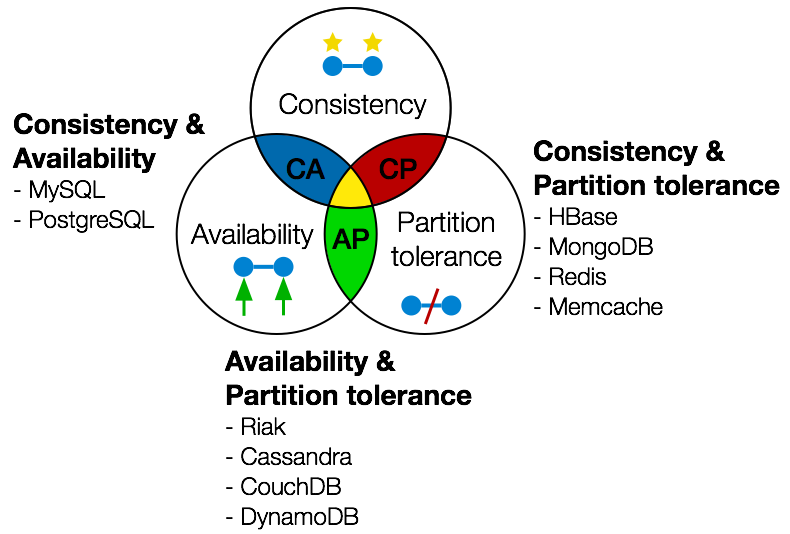
\includegraphics[width=0.9\textwidth]{gfx/CAPTheorem.png}
  \caption{\label{fig:captheorem}Clasificación de bases de datos mediante el teorema de CAP.}
\end{figure}

\section{Tipos de bases de datos NoSQL}

En esta sección vamos a caracterizar las bases de datos NoSQL según la forma en la que almacenan los datos. Podemos clasificar la mayoría de bases de datos NoSQL en alguna de las siguientes 4 categorías, como se describe en la propia documentación de MongoDB \cite{mongoclassification}.

\begin{itemize}
    \item \texttt{Almacenamiento clave-valor}: Son grandes tablas que almacenan la información en forma de clave-valor. Las bases de datos de este tipo más populares son: RedisDB, Riak y Voldemort.
    \item \texttt{Almacenamiento basado en documentos}: Es este tipo de bases de datos, los datos se almacenan en forma de documentos. El concepto de documento depende de la definición de la base de datos, normalmente son grandes conjuntos de claves-valor codificados o encapsulados como un tipo de documento. En esta categoría, MongoDB es el más popular y más usado, pero existen otros como CouchDB.
    \item \texttt{Almacenamiento basado en grafos}: Estas bases de datos almacenan relaciones en forma de grafos. Algunas de las bases de datos más populares son: Neo4j y FlockDB.
    \item \texttt{Almacenamiento en columnas}: En este tipo de bases de datos, se almacenan columnas en lugar de filas como en el resto de tipos. Está optimizado para grandes volúmenes de datos. Las bases de datos más populares de este tipo son: Cassandra y HBase. 
\end{itemize}

En el artículo \cite{nosqlcomparativas}, puede verse una comparativa entre distintas bases de datos NoSQL sobre lenguaje en el que están escritas, ternologías que utilizan, tipo de base de datos, etc.

\section{Comparativa NoSQL con SGBDR}

En esta sección vamos a realizar una comparativa entre las bases de datos SQL y NoSQL.

En primer lugar, además de las dos diferencias comentadas anteriormente, es de destacar, que las bases de datos NoSQL son libres de esquema, esto es, que no necesitan una planificación antes de empezar a almacenar datos a nivel de relaciones, tablas, etc. Los datos almacenados son independientes entre ellos y pueden ser totalmente distintos. Esto aporta un gran valor en el sentido de adaptabilidad a nuevos cambios.

\subsection{Sistemas de Gestión de Bases de Datos Relacionales}

Vamos a dar algunas características que caracterizan a Sistemas de Gestión de Bases de Datos Relacionales (SGBDR), para comenzar veremos algunos de las ventajas que presentan de este tipo de base de datos:

\begin{itemize}
    \item Mayor soporte y herramientas debido a su amplia presencia en el mercado.
    \item Permiten combinar diferentes tablas eficientemente para obtener información relacionada.
    \item Los datos siguen una estructura predefinida en los esquemas.
    \item Proporcionan atomicidad en las operaciones y transaccionalidad entre tablas, esto evita que queden datos inconsistentes si se produce un error en cualquier punto de una operación.
\end{itemize}

Como inconvenientes señalar:

\begin{itemize}
    \item No son flexibles, en el sentido de que los datos tienen que seguir el esquema definido y tienen que estar correctamente validados.
    \item Incremento del procesamiento con el incremento de la complejidad en las relaciones.
    \item Dificultad para escalar, habitualmente necesitan de ampliaciones costosas de hardware.
\end{itemize}

\subsection{Bases de Datos NoSQL}

Una de las principales características que tendría el conjunto de bases de datos NoSQL, es que proporcionan una manera alternativa de almacenar la información y muy diversa por los tipos que comentamos anteriormente, por tanto, ya nos proporcionan una cierta ventaja de flexibilidad que no tenemos con los sistemas SGBDR tradicionales. Veamos ahora algunas características favorables que poseen las bases de datos NoSQL:

\begin{itemize}
    \item Escalabilidad. En general, tienen buen escalamiento horizontal.
    \item Soporte para modelos flexibles, libres de esquemas, tipos y validaciones.
    \item Optimizadas para grandes volúmenes de datos.
    \item Precisan de menos recursos para su funcionamiento.
\end{itemize}

Por contra:

\begin{itemize}
    \item No todas garantizan la atomicidad y consistencia en los datos.
    \item Falta de estandarización. No existe lenguaje un estándar para estas bases de datos, al contrario que ocurre con las BD Relacionales que todas usan SQL.
    \item Falta de herramientas de gestión. Muchas de ellas solo son accesibles por consola.
\end{itemize}

\section{MongoDB}

En esta sección vamos a centrarnos en la base de datos NoSQL más popular hasta el momento, MongoDB es una base de datos orientada a documentos muy usada para técnicas de Big Data. Toda esta sección está extraida de la documentación oficial de MongoDB \cite{mongodb}.

Las principales características son:

\begin{itemize}
    \item MongoDB es una base de datos \textit{open source}, escrita en C++, lo que favorece su rapidez y le proporciona un buen rendimiento.
    \item Es una base de datos distribuida en su núcleo, por lo que se escala horizontalmente de forma fácil, permite la distribución geográfica y una alta disponibilidad.
    \item Almacenamiento de modelo de datos flexibles. Basada en documentos en forma de JSON, permite indexación y operaciones de agregación.
    \item Garantiza transacciones ACID (atomicidad, consistencia, aislamiento y durabilidad) en multidocumentos. Esta reciente característica ha sido integrada en la versión 4.0 de MongoDB.
\end{itemize}

\subsection{Modelo de datos}\label{datamodelmongo}

MongoDB nos provee de un modelo de datos flexible, esto nos permite almacenar desde un documento simple de parejas clave-valor, hasta un documento con subdocumentos embebidos y/o arrays complejos a varios niveles de profundidad.

Posee una sintaxis para realizar consultas muy variada, nos permite hacer consultas simples, con un lenguaje muy descriptivo, sofisticados \textit{pipeline} para consulta, transformación y explotación de datos, búsquedas facetadas, etc.

MongoDB almacena los datos en formato BSON \cite{bsonspec} que es una extensión de los objetos nativos de JavaScript (JSON) a los que añade algunos tipos de datos extra. Estos tipos de datos, se asemejan a los objetos que encontramos en los distintos lenguajes de programación, lo que hace que se produzca una rápida adaptación y una fácil integración con el modelo de datos de MongoDB.

Una de las principales diferencias con las bases de datos relacionales a la hora de modelizar, es que, mientras que en las bases de datos relaciones es habitual crear distintas tablas para trabajar mediante JOINs, en MongoDB es habitual tener todos los datos necesarios para un registro en un mismo documento, lo que reduce la complejidad de tener que realizar JOINs entre tablas y ayuda a la mejora del rendimiento de las consultas.

\subsection{Tipos de consultas}

MongoDB tiene distintos métodos para la consulta y explotación de los datos almacenados:

\begin{itemize}
    \item Clave-valor: Búsquedas simples en cualquier campo del documento.
    \item Rangos: Es posible utilizar los operadores de desigualdades (mayor que, menor que...) para hacer búsquedas por rango y obtener un subconjunto de documentos que satisfagan las condiciones.
    \item Búsquedas Geoespaciales: Devuelven resultados basados en proximidad a ciertos criterios.
    \item Búsquedas de resutlados en un orden relevante, o en búsquedas facetadas. Es posible utilizar operadores lógicos (and, or...), agrupar, contar resultados, etc.
    \item Operadores de agregación: Permite hacer consultas y transformaciones de los datos almacenados. Provee una interfaz completa de operadores dedicados (operaciones lógicas, desigualdades, proyecciones...). En este trabajo, veremos la implementación de consultas de bases de conjuntos difusos sobre este operador de agregación.
    \item JOINs y grafos: con el operador \textit{lookup} podemos hacer JOIN entre colecciones, y con el operador \textit{graphLookup} mongo provee una forma nativa de procesar grafos, árboles y estructuras jerárquicas.
\end{itemize}


\subsection{Indexación}

Según se define en la propia documentación de MongoDB \cite{mongodb}, <<\textit{la indexación es un mecanismo crucial para la optimización del rendimiento y escalabilidad del sistema mientras provee un acceso flexible a tus datos}>>. Mongo permite la indexación en cualquier campo del documento, incluso en los campos de un array.

Mongo provee la facilidad para crear índices compuestos, únicos, array, índices geoespaciales, hash y texto.

Además, la intersección de índices permite a MongoDB usar más de un índice para la optimización de las consultas.

\subsection{Agregación}

Una de las características más importantes de MongoDB a la hora de explotar y transformar datos son las agregaciones. Esta base de datos nos provee dos formas de realizarla, mediante \textit{map-reduce} y mediante \textit{pipeline}.

\subsubsection{Map-Reduce}\label{mapreduce}

Map-Reduce es un modelo de programación general muy utilizado para trabajar con grandes volúmenes de datos y poder introducir paralelismo. MongoDB provee un comando para utilizarlo directamente sobre la base de datos de forma nativa.

El modelo map-reduce, consiste en generar un subconjunto de documentos útiles preprocesando un conjunto más amplio previamente y agrupando en una última etapa. Puede encontrarse más información de este comando y sus usos en \href{https://docs.mongodb.com/manual/core/map-reduce/}{la documentación oficial}.

\subsubsection{Pipeline}\label{pipeline}

La segunda forma para implementar operaciones de agregación es mediante el framework \textit{pipeline}. Con este comando los documentos son procesados mediante una secuencia ordenada de etapas, donde cada etapa recibe una colección de documentos procesados por la etapa anterior, los procesa y los envía como entrada de la siguiente etapa, así hasta producir el resultado final. Mediante este operador, el filtrado de documentos sobre una colección de documentos se haría usando el operador \textit{match} en la etapa correspondiente del \textit{pipeline} de agregación.

Las etapas permitidas para este operador se pueden encontrar en la \href{https://docs.mongodb.com/manual/reference/operator/aggregation-pipeline/}{documentación del operador}. En nuestra propuesta se proporciona una serie de operadores adicionales que se pueden utilizar en las etapas de \textit{match} y \textit{projection}.

La etapa \textbf{match}, como se describe en su propia documentación, sirve para filtrar los documentos que van a pasar a la siguiente etapa. Selecciona aquellos que cumplan ciertas condiciones descritas mediante los operadores\footnote{https://docs.mongodb.com/manual/reference/operator/aggregation/} permitidos para esta etapa. Los operadores que hemos extendido para trabajar con datos difusos son:

\begin{itemize}\label{mongooperators}
    \item \textbf{\$eq}: selecciona los documentos cuyo valor coincida con el especificado.
    \item \textbf{\$gt}: selecciona los documentos cuyo valor sea mayor que el especificado.
    \item \textbf{\$gte}: selecciona los documentos cuyo valor sea mayor o igual que el especificado.
    \item \textbf{\$lt}: selecciona los documentos cuyo valor sea menor que el especificado.
    \item \textbf{\$lte}: selecciona los documentos cuyo valor sea menor o igual que el especificado.
\end{itemize}

Además de estos, vamos a ver los que nos serán de utilidad para su implementación:

\begin{itemize}
    \item \textbf{\$and}: Operador lógico, recibe una lista de expresión y filtra aquellos documentos que cumplan con todas ellas.
    \item \textbf{\$or}: Operador lógico, recibe una lista de expresión y filtra aquellos documentos que cumplan al menos una de ellas.
    \item \textbf{\$add}: Operador aritmético, recibe una lista de expresiones, que deben de ser evaluadas como un número, y suma todas ellas.
    \item \textbf{\$substract}: Operador aritmético, recibe una lista de expresiones, que deben de ser evaluadas como un número, y resta todas ellas.
    \item \textbf{\$multiply}: Operador aritmético, recibe una lista de expresiones, que deben de ser evaluadas como un número, y multiplica todas ellas.
    \item \textbf{\$divide}: Operador binario aritmético, recibe una lista de 2 expresiones y devuelve la división del primero de ellos entre el segundo.
    \item \textbf{\$cond}: Operador ternario condicional, recibe una lista de 3 expresiones y permite evalua la segunda o la tercera en función del resultado obtenido en la primera. Este operador nos permite realizar los clásicos \textit{if-else} de cualquier lenguaje de programación.
    \item \textbf{\$arrayElemAt}: Operador para expresiones con arrays. Recibe una lista de 2 expresiones, donde el primer parámetro es el campo que corresponde con el array y la segunda es el índice del array que se quiere obtener. Devuelve el valor que se encuentre en la posición solicitada del array.
    \item \textbf{\$expr}\footnote{\url{https://docs.mongodb.com/manual/reference/operator/query/expr/}}: El operador ``expr'' es un operador de consultas, permite el uso\footnote{Uso de operador expr con expresiones condicionales: \url{https://docs.mongodb.com/manual/reference/operator/query/expr/\#using-expr-with-conditional-statements}} de expresiones de agregación en el lenguaje de consultas. El uso que nos interesa es el combinado con el operador ``\$cond''.
\end{itemize}

La etapa \textbf{projection} sirve para establecer que campos mostrar de la colección resultante. Nos permite tanto eliminar campos del propio documento, como generar y visualizar campos nuevos. En esta parte nos hemos centrado en ampliar la posibilidad de proyectar el grado de cumplimiento para los campos difusos.

En el capítulo \ref{propuesta} veremos estos operadores y la propuesta realizada para ampliar estas etapas.


\chapter{Conjuntos Difusos}
\input{chapters/Fuzzy.tex}

\part{Conclusiones}

\chapter{Conclusiones y vías futuras}
\input{chapters/Conclusions.tex}

% ********************************************************************
% Backmatter
%*******************************************************
%\appendix
%\renewcommand{\thechapter}{\alph{chapter}}
%\cleardoublepage
%\include{Chapters/Chapter0A}
%********************************************************************
% Other Stuff in the Back
%*******************************************************
\cleardoublepage%********************************************************************
% Bibliography
%*******************************************************
% work-around to have small caps also here in the headline
\manualmark
\markboth{\spacedlowsmallcaps{\bibname}}{\spacedlowsmallcaps{\bibname}} % work-around to have small caps also
%\phantomsection 
\refstepcounter{dummy}
\addtocontents{toc}{\protect\vspace{\beforebibskip}} % to have the bib a bit from the rest in the toc
\addcontentsline{toc}{chapter}{\tocEntry{\bibname}}
\label{app:bibliography}
\printbibliography

\cleardoublepage%*******************************************************
% Declaration
%*******************************************************
\refstepcounter{dummy}
\pdfbookmark[0]{Declaration}{declaration}
\chapter*{Declaración}
\thispagestyle{empty}

% TODO - DNI
Yo, \myName, alumno de la titulación \emph{\myDegree} de la \emph{\myFaculty} y de la \emph{\myOtherFaculty} de la \emph{\myUni}, con DNI XXXXXXXXX, asumo la originalidad de este trabajo, entendida en el sentido de que no se han utilizado fuentes sin citarlas debídamente.

Y para que conste, expido y firmo la presente declaración.

\bigskip
 
\noindent\textit{\myLocation, } %TODO - DATE

\smallskip

\begin{flushright}
    \begin{tabular}{m{5cm}}
        \\ \hline
        \centering\myName \\
    \end{tabular}
\end{flushright}
\cleardoublepage\pagestyle{empty}

\hfill

\vfill


\pdfbookmark[0]{Colophon}{colophon}
\section*{Colophon}
This document was typeset using the typographical look-and-feel \texttt{classicthesis} developed by Andr\'e Miede. 
The style was inspired by Robert Bringhurst's seminal book on typography ``\emph{The Elements of Typographic Style}''. 
\texttt{classicthesis} is available for both \LaTeX\ and \mLyX: 
\begin{center}
\url{https://bitbucket.org/amiede/classicthesis/}
\end{center}
Happy users of \texttt{classicthesis} usually send a real postcard to the author, a collection of postcards received so far is featured here: 
\begin{center}
\url{http://postcards.miede.de/}
\end{center}
 
\bigskip

\noindent\finalVersionString

%Hermann Zapf's \emph{Palatino} and \emph{Euler} type faces (Type~1 PostScript fonts \emph{URW
%Palladio L} and \emph{FPL}) are used. The ``typewriter'' text is typeset in \emph{Bera Mono}, 
%originally developed by Bitstream, Inc. as ``Bitstream Vera''. (Type~1 PostScript fonts were made 
%available by Malte Rosenau and
%Ulrich Dirr.)

%\paragraph{note:} The custom size of the textblock was calculated
%using the directions given by Mr. Bringhurst (pages 26--29 and
%175/176). 10~pt Palatino needs  133.21~pt for the string
%``abcdefghijklmnopqrstuvwxyz''. This yields a good line length between
%24--26~pc (288--312~pt). Using a ``\emph{double square textblock}''
%with a 1:2 ratio this results in a textblock of 312:624~pt (which
%includes the headline in this design). A good alternative would be the
%``\emph{golden section textblock}'' with a ratio of 1:1.62, here
%312:505.44~pt. For comparison, \texttt{DIV9} of the \texttt{typearea}
%package results in a line length of 389~pt (32.4~pc), which is by far
%too long. However, this information will only be of interest for
%hardcore pseudo-typographers like me.%
%
%To make your own calculations, use the following commands and look up
%the corresponding lengths in the book:
%\begin{verbatim}
%    \settowidth{\abcd}{abcdefghijklmnopqrstuvwxyz}
%    \the\abcd\ % prints the value of the length
%\end{verbatim}
%Please see the file \texttt{classicthesis.sty} for some precalculated 
%values for Palatino and Minion.
%
%    \settowidth{\abcd}{abcdefghijklmnopqrstuvwxyz}
%    \the\abcd\ % prints the value of the length
% ********************************************************************
% Game Over: Restore, Restart, or Quit?
%*******************************************************
%\listoftodos
\end{document}
% ********************************************************************